\chapter{混合策略纳什均衡}  \label{c6}

策略型博弈并不总是存在纯策略均衡，即每个参与者都确定地选择他的纯策略。在本章中，我们将展示纳什（1951年）的经典结论：如果允许参与者采用混合策略，则任何有限策略型博弈都必然存在均衡。所谓混合策略，是指参与者按照某种概率分布在给定的纯策略之间进行随机化选择。若在某一混合策略组合下，没有任何参与者能够通过单方面改变其策略来提升其期望效用，则该组合被称为混合策略均衡。

在本章中，我们简要回顾第5章的相关内容，即参与者的收益如何通过期望效用函数来体现他对随机结果的偏好。作为示例，我们考虑一个单人决策问题：是否遵守某项法律要求。随后，我们将该问题转化为一个博弈，即监管者（参与者 I）与被监管者（参与者 II）之间的监管博弈。该博弈在纯策略下没有均衡。然而，在这个博弈中，主动随机化自然而然地出现，因为监管者只会在部分情况下选择检查。该博弈的混合策略纳什均衡很好地展示了混合策略纳什均衡的很多特征，尤其是参与者的随机化概率依赖于对方的收益。

接着，我们讨论一般的两人策略型博弈（在第 3 章中已经讨论过），此处称为双矩阵博弈。两个参与者的收益用矩阵形式表示，能够通过与概率向量（即参与者的混合策略）相乘来方便地计算期望收益。混合策略作为概率向量，还具有几何上的解释，我们将详细阐述(并在第9章进一步展开)。从几何角度看，利用概率对纯策略进行混合等同于取这些策略的凸组合。

在两人博弈中，我们通常将参与者命名为I和II，并将他们的纯策略分别表示为行 \(i = 1,\ldots,m\) 和列 \(j = 1,\ldots ,n\)。在 \(N\) 人博弈中，我们采用最常用的记号，将参与者编号为 \(i = 1,\ldots,N\)。

最优反应条件为某一混合策略在何时是对另一个参与者（或在多于两人时，对所有其他参与者）的混合策略的最优反应，提供了一种简洁且有限的条件。即，对于属于最优反应的混合策略，只有那些属于最优反应的纯策略才可能以正概率被选择。所有作为最优反应的纯策略的期望收益均达到最大值，并且相等。纳什(1951，第287页)将其表述为一个“平凡条件”，而且确实不难证明(见命题6.1)。然而，最优反应条件对于理解和计算混合策略均衡至关重要。

在第6.5节中，我们陈述并证明纳什定理，即每个博弈都存在一个均衡。我们遵循纳什的原始证明(为简化表示，针对两人博弈)，并陈述并简要说明该证明中使用的布劳威尔不动点定理。在第7章中，我们将证明这一不动点定理。

最后，第6.6 - 6.8节展示如何找到双矩阵博弈的均衡，特别是当一个参与者只有两种策略时。

零和博弈这一特殊且有趣的博弈将在第8章中讨论。

\section{预备知识和学习目标}  \label{sec6.1}

预备知识是熟悉第3章的内容，并知道收益仅在正仿射变换下是唯一的，如第5章所讨论的。熟练掌握矩阵乘法将十分有用，我们也会把它作为背景知识进行回顾。我们还需要理解图 5.4 中所介绍的线段的代数表示方法。

学习本章后，你应该能够:

\begin{itemize}
\item 解释什么是混合策略和混合策略纳什均衡；
\end{itemize}

\begin{itemize}
\item 陈述关于混合策略的主要定理，即最优反应条件和纳什关于混合策略纳什均衡存在性的定理；
\end{itemize}

\begin{itemize}
\item (作为一项重要技能)使用“差分技巧”，必要时使用上包络法，找出小型双矩阵博弈的所有混合策略纳什均衡；
\end{itemize}

\begin{itemize}
\item 给出退化博弈的定义，并找出小型退化博弈的所有均衡。
\end{itemize}

\section{监管博弈}  \label{sec6.2}

在本节中，我们考虑一个两人监管博弈，其中随机或混合策略自然出现。当一个参与者采用混合策略时，另一个参与者面对的是一个“彩票”，其结果需要根据期望收益来评估，这一点已在第5章中进行了详细讨论。

简要回顾一下，图\ref{fig:6.1}展示了一个单人{\color{red}游戏}：该参与者可以选择遵守法律要求(如购票乘车)，或者选择违规。若她选择遵守，则收益为0。若选择违规，则有10\%的概率被抓住并支付罚款，此时收益为 $-90$，另外有90\%的概率获得收益10。根据这些数值，违规会导致一个随机结果，其期望收益为 \({0.9} \cdot  {10} + {0.1} \cdot  \left( {-{90}}\right)=0\)。因此，参与者对这两种选择之间无差异。实际上，假设收益0和10这两种结果分别被设定为效用函数的原点和单位，那么“被抓住”的效用 $-90$ 就是由选择无差异性决定的。如果参与者在被抓住的概率为4\%时，其选择无差异，那么 $-90$ 需替换为 \(- u\) ，并使得
\[
0 = {0.96} \cdot  {10} + {0.04} \cdot  \left( {-u}\right) ,
\]
于是，\(u = {9.6}/{0.04} = {240}\)。此外，请注意，效用函数的原点和单位是任意的，它们可以通过正仿射变换进行改变。例如， \(0,{10}, - {90}\) 可以替换为 \(0,1, - 9\) 或 \(- 1,0, - {10}\)。

\begin{figure}[htbp]
  \centering
  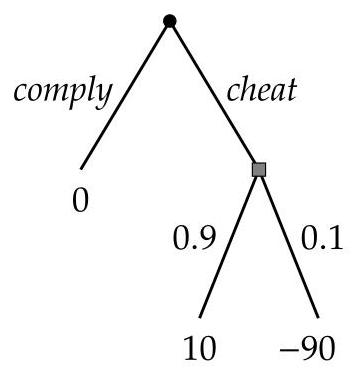
\includegraphics[width=0.3\textwidth]{images/ch06-fig01.jpg}
  \caption{遵守与违规之间的单人决策问题。在给定的收益下，参与者无差异。}
  \label{fig:6.1}
\end{figure}



在实践中，参与者的风险偏好可能是未知的。利用博弈论分析时，应针对不同的收益参数设定进行考察，以检验这些参数对结果的影响程度。

我们现在考虑监管博弈。对于参与者II，即被监管者，“遵守”策略意味着履行某些法律义务(如购买交通票或纳税)。被监管者有动机通过选择“违规”来违反这些义务。参与者I，即监管者，应该核实被监管者是否遵守规定，但这样做需要付出成本进行检查。如果监管者进行检查并抓住被监管者违规，那么被监管者必须支付罚款。

图\ref{fig:6.2}展示了监管博弈的可能收益情况。当监管者选择“不检查”且被监管者选择“遵守”时，双方的收益均为 0。如果监管者不检查，则被监管者倾向于“违规”，其收益为10，而监管者的收益为 $-10$。监管者也可以选择“检查”。如果被监管者选择“遵守”，则检查不会改变她的收益0，而监管者需要承担检查成本，其收益为 $-1$。如果被监管者选择“违规”，检查将使其支付罚款（参与者 II 的收益为 $-90$），同时仍会给监管者带来一定的不便（参与者 I的收益为 $-6$）。

\begin{figure}[htbp]
  \centering
  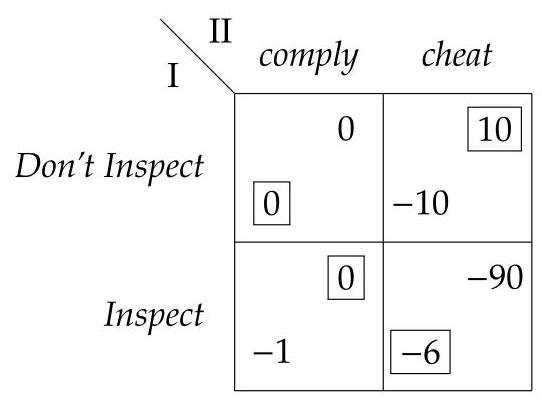
\includegraphics[width=0.4\textwidth]{images/ch06-fig02.jpg}
  \caption{监管者（参与者 I）与被监管者（参与者 II）之间的监管博弈。}
  \label{fig:6.2}
\end{figure}

在所有情况下，参与者I非常希望参与者II遵守规定，但这不在参与者I的控制范围内。然而，如图\ref{fig:6.2}中收益 $-6$ 的最优反应框所示，如果被监管者违规，监管者更倾向于检查(因为 $-6$ 优于 $-10$)。如果监管者始终偏好“不检查”，那么“不检查”将成为一种占优策略，并构成一个（唯一）均衡，在该均衡中被监管者选择“违规”。

图\ref{fig:6.2}中的最优反应收益表明，这个博弈在纯策略中没有均衡。如果任何一个参与者确定了一个确定性的选择(如参与者I选择“不检查”)，那么另一个参与者的最优反应是唯一的(这里是参与者II选择违规)，而最初的选择并不是对这个最优反应的最优反应(当另一个参与者违规时，参与者I更倾向于检查，而参与者II则更倾向于遵守)。均衡中的策略必须是相互的最优反应，因此在这个博弈中，任何一对纯策略都无法满足这一条件。

在图\ref{fig:6.2}的博弈中，参与者应该怎么做呢？一种可能性是他们为最坏的情况做准备，即选择所谓的极大极小策略。极大极小策略是在对手所有可能的选择下，最大化参与者的最差收益。参与者 \(\mathrm{I}\) 的极大极小策略(作为纯策略)是检查(监管者可以保证自己的收益为 -6)，而参与者II的极大极小策略是遵守(这可以保证她的收益为0)。然而，这不是一个均衡，因此也不是给两个参与者的稳定建议，因为参与者I可以将他的策略改为“不检查”来提高他的收益。

在这个博弈中，参与者I的混合策略是以一定概率进行检查。在检查的情境下，随机化也是一种降低成本的实用方法。即使检查不是必然的，被抓住的可能性足够高也应该能阻止被检查者作弊。

参与者I的混合策略是为“检查”设定一个概率 \(p\) ，因此“不检查”的概率为 \(1 - p\) 。现在，参与者I可以选择一个概率 \(p \in  \left\lbrack  {0,1}\right\rbrack\) ，而不是他的两种纯策略。这包括当 \(p = 0\) 时的纯策略“不检查”和当 \(p = 1\) 时的纯策略“检查”。参与者II的混合策略是为“作弊”设定一个概率 \(q\) ，为“遵守”设定一个概率 \(1 - q\) 。这样，她在两种纯策略之间的选择就扩展到了对 \(q \in  \left\lbrack  {0,1}\right\rbrack\) 的任何选择。实际上，这意味着参与者现在各自有一个无限的策略集 \(\left\lbrack  {0,1}\right\rbrack\) ，其收益按期望效用计算。这个新的博弈被称为原 \(2 \times  2\) 博弈的混合扩展。

策略对 \(\left( {p,q}\right)  \in  \left\lbrack  {0,1}\right\rbrack   \times  \left\lbrack  {0,1}\right\rbrack\) 何时构成一个均衡(将其称为混合策略纳什均衡？这些策略必须是彼此的最优反应。假设参与者I选择 \(p\) ，参与者II必须确定她的最优反应。我们首先考虑她可能的纯反应。她选择“遵守”的期望效用是 \(\left( {1 - p}\right)  \cdot  0 + p \cdot  0 = 0\) ，这与 \(p\) 无关。她选择“作弊”的期望效用是 \(\left( {1 - p}\right)  \cdot  {10} + p \cdot  \left( {-{90}}\right)  = {10} - {100p}\) 。实际上，参与者II面临着图\ref{fig:6.1}中的决策情形，其中0.9和0.1分别被 \(1 - p\) 和 \(p\) 取代。显然，当 \(0 > {10} - {100p}\) 时，即 \(p > {0.1}\) 时，她更倾向于“遵守”；当 \(0 < {10} - {100p}\) 时，即 \(p < {0.1}\) 时，她更倾向于“作弊”；当且仅当 \(0 = {10} - {100p}\) 时，即 \(p = {0.1}\) 时，她无差异。

在混合扩展中，参与者 II 也可以通过选择 \(q\) 进行混合，使得 \(0 < q < 1\) 。我们断言，只有当她无差异时才会出现这种情况。也就是说，假设 \(p\) 非常低，例如 \(p = {0.01}\) ，那么作弊的期望效用为 \({0.99} \cdot  {10} + {0.01} \cdot  \left( {-{90}}\right)  = 9\) 。采用混合策略 \(q\) 时，参与者 II 的期望效用为 \(0 \cdot  \left( {1 - q}\right)  + {9q} = {9q}\) ，显然当 \(q = 1\) 时该期望效用达到最大化，这是她的纯最优反应——作弊。类似地，如果 \(p\) 很高，例如 \(p = {0.2}\) ，那么作弊的期望效用为 \({0.8} \cdot  {10} + {0.2} \cdot  \left( {-{90}}\right)  =  - {10}\) 。采用混合策略 \(q\) 时，参与者 II 的期望效用为 \(0 \cdot  \left( {1 - q}\right)  - {10q} =  - {10q}\) ，当 \(q = 0\) 时期望效用达到最大化，这是她的纯最优反应——遵守规则。只有当遵守规则和作弊带来相同的期望效用时，参与者 II 的期望效用才不依赖于 \(q\) ，实际上她可以选择任何 \(q \in  \left\lbrack  {0,1}\right\rbrack\) 作为最优反应。图 6.3 展示了最优反应概率 \(q\) 相对于 \(p\) 的关系图。

\begin{figure}[htbp]
  \centering
  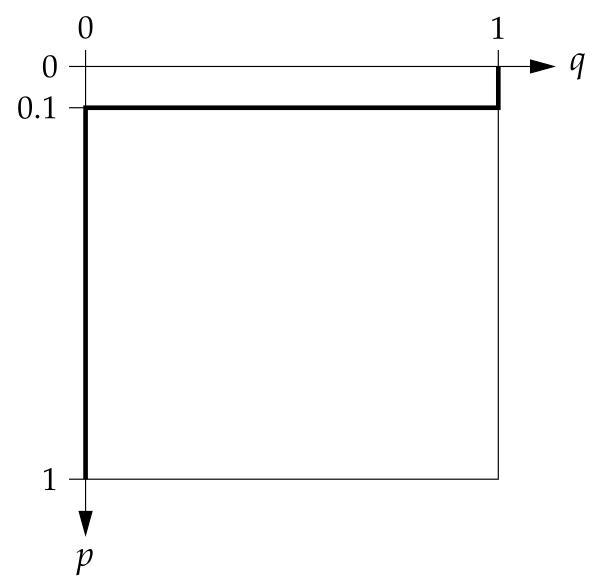
\includegraphics[width=0.4\textwidth]{images/ch06-fig03.jpg}
  \caption{监管博弈中参与者 II 作弊的最优反应混合策略概率 $q$（黑线）与参与者 I 检查的混合策略概率 $p$ 的关系图。混合策略方块的绘制使得其角点与图~\ref{fig:6.2} 中的四个单元格相对应。}
  \label{fig:6.3}
\end{figure}


综上所述，参与者 II 可能在其纯策略之间进行随机选择的唯一情况是，两种策略给她带来相同的期望效用。正如下面命题 6.1 所陈述{\color{red}并}正式证明的那样，对于给定的其他参与者的混合策略，参与者对劣于其他纯策略的纯策略赋予正概率永远不是最优的。

\begin{figure}[htbp]
  \centering
  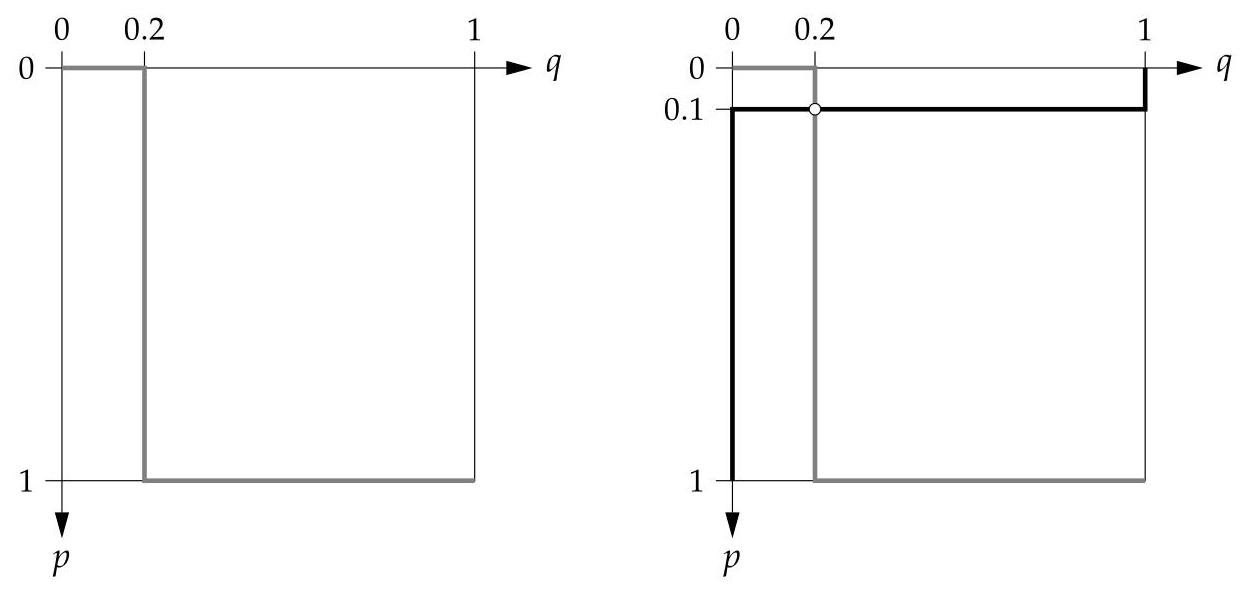
\includegraphics[width=0.9\textwidth]{images/ch06-fig04.jpg}
  \caption{左图：参与者 I 相对于 $q$ 的最优反应混合策略概率 $p$（灰线）。右图：两条最优反应线的交点确定了唯一的混合策略纳什均衡，其中 $p=0.1$ 且 $q=0.2$。}
  \label{fig:6.4}
\end{figure}


类似地，考虑参与者 II 的一种混合策略，她以概率 \(q\) 作弊。参与者 I 的纯策略的期望效用分别为:不检查时为 \(- {10q}\) ，检查时为 \(\left( {-1}\right) \left( {1 - q}\right)  - {6q} =  - 1 - {5q}\) 。如果参与者 I 以概率 \(p\) 选择检查，那么他的期望效用为 \(\left( {-{10q}}\right) \left( {1 - p}\right)  + \left( {-1 - {5q}}\right) p =  - {10q} + p\left( {{5q} - 1}\right)\) 。这是关于 \(p\) 的线性函数，若 \({5q} - 1 < 0\) ，即 \(q < {0.2}\) ，则在 \(p = 0\) 处达到最大值；若 \({5q} - 1 > 0\) ，即 \(q > {0.2}\) ，则在 \(p = 1\) 处达到最大值；只有当 \(q = {0.2}\) 时，它才不依赖于 \(p\) ，此时 \(p \in  \left\lbrack  {0,1}\right\rbrack\) 可以任意选择。这在图\ref{fig:6.4} 的左图中有所展示。

图\ref{fig:6.4}中的右图展示了当两个混合策略互为最优反应时，两条最优反应线的交点，该交点对应着博弈在 \(p = {0.1}\) 和 \(q = {0.2}\) 处的唯一混合策略纳什均衡。它与图3.10中用于古诺双寡头博弈的最优反应示意图相似，只是顺时针旋转了四分之一圈，以便垂直和水平参数 \(p\) 和 \(q\) 与图\ref{fig:6.2}中 \(2 \times  2\) 博弈的行和列相匹配。

在监管博弈的 \(p = {0.1}\) 和 \(q = {0.2}\) 唯一混合策略纳什均衡中，期望效用为

\[
\begin{aligned}
&\text{对于玩家 I:} &
-10q &= -1(1-q)-6q = -2,\\
&\text{对于玩家 II:} &
0 &= 10(1-p)-90p = 0.
\end{aligned}
\]

均衡概率 \(q\) 和 \(p\) 由这些方程(独立地)确定。值得注意的是，它们取决于对手的收益，而非参与者自身的收益(因此，只要图\ref{fig:6.2}中的循环偏好结构保持不变，参与者自身的收益就可以改变)。例如，人们可能认为，被抓后处以比 -90 更严厉的惩罚会降低均衡状态下作弊的概率。实际上并非如此。真正改变的是检查的概率 \(p\) ，该概率会降低，直到被检查者感到无差异为止。

这种对对手收益的依赖是混合策略纳什均衡最违反直觉的特性。此外，当参与者在均衡状态下感到无差异时，混合策略本身似乎也自相矛盾。例如，如果参与者 II 可以同样地选择遵守规则或作弊，那她为什么要随机选择呢？特别是，她可以选择遵守规则并确定获得零收益，这样既简单又安全。答案是，正是因为没有动机去选择一种策略而非另一种策略，参与者才可以采用混合策略，而且只有在这种情况下才可能存在均衡。如果参与者 II 确定会遵守规则，那么参与者 \(\mathrm{I}\) 的唯一最优选择就是不进行检查，但这样一来，遵守规则就不是最优选择了，所以这不是一个均衡。

\section{双矩阵博弈}   \label{sec6.3}

接下来，我们将讨论策略形式下一般博弈的混合策略纳什均衡。对于两人博弈，大多数概念可以用更简单的符号来解释。此时，参与者I和参与者II的策略分别对应一个表格的行和列，每个单元格中有两个收益值，因此该博弈由两个收益矩阵定义。有关矩阵运算的一些基本事实可在背景材料中找到。

背景材料:矩阵乘法

如果 \(A\) 是一个 \(m \times  k\) 矩阵， \(B\) 是一个 \(k \times  n\) 矩阵，那么它们的矩阵乘积 \(A \cdot  B\) (或简记为 \({AB}\) )是一个 \(m \times  n\) 矩阵 \(C\) ，其元素为：
\begin{equation}\label{eq:6.1}
c_{ij} = \sum_{s=1}^{k} a_{is} b_{sj}, \quad 
(1 \le i \le m, \; 1 \le j \le n).
\end{equation}


写矩阵乘积 \({AB}\) 时，其前提是该乘积是有定义的，即 \(A\) 的列数等于 \(B\) 的行数。矩阵乘法满足结合律，即对于矩阵 \(A,B,C\) ，有 \(\left( {AB}\right) C = A\left( {BC}\right)\)，可将其简记为 \({ABC}\)。

在处理矩阵时，我们始终使用以下符号。这里考虑的所有矩阵都是实矩阵(元素属于 \(\mathbb{R}\) )。 \(m \times  n\) 矩阵的集合记为 \({\mathbb{R}}^{m \times  n}\) 。 \(m \times  n\) 矩阵 \(A\) 的转置记为 \({A}^{\top }\) ，它是一个 \(n \times  m\) 矩阵。若 \(A\) 的元素为 \({a}_{ij}\) ，则 \({A}^{\top }\) 的元素为 \({a}_{ji}\) ，其中 \(1 \leq  i \leq  m,1 \leq  j \leq  n\) 。

所有向量均为列向量，因此如果 \(x \in  {\mathbb{R}}^{n}\) ，那么 \(x\) 是一个 \(n \times  1\) 矩阵， \({x}^{\top }\) 是 \({\mathbb{R}}^{1 \times  n}\) 中对应的行向量，并且通过转置符号可以很容易识别出行向量。向量 \(x \in  {\mathbb{R}}^{n}\) 的分量为 \({x}_{1},\ldots ,{x}_{n}\) 。我们将 \({\mathbb{R}}^{n}\) 中两个向量 \(x,y\) 的标量积(scalar product)写成矩阵乘积 \({x}^{\top }y\) 。用图形表示(每个矩阵元素用一个方块表示，这里是 \(n = 4\) ):

\begin{equation}\label{eq:6.2}
\vcenter{\hbox{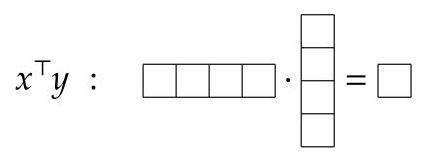
\includegraphics[width=0.3\textwidth]{images/ch06-fig05.jpg}}}
\end{equation}

我们尽可能使用矩阵乘法。特别地，标量被视为 \(1 \times  1\) 矩阵。列向量 \(x\) 从右侧与标量 \(\lambda\) 相乘，行向量 \({x}^{\top }\) 从左侧与标量 \(\lambda\) 相乘。

\begin{equation}\label{eq:6.3}
\vcenter{\hbox{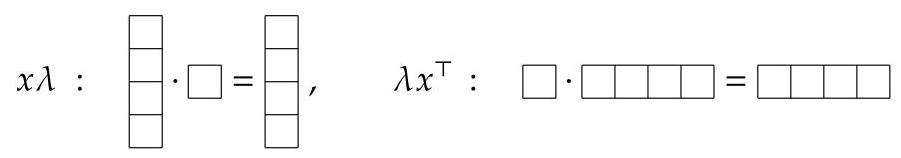
\includegraphics[width=0.7\textwidth]{images/ch06-fig06.jpg}}}
\end{equation}

更多详细信息请参阅矩阵乘法可视化的背景材料。

\(\Rightarrow\) 练习~\ref{exer:6.1} 比较了 \({x}^{\top }y\) 和 \(x{y}^{\top }\) 。

此外，特殊向量$\mathbf{0}$和$\mathbf{1}$表示它们的所有分量分别等于0和1，其维度取决于具体情境。像 \(x \geq  \mathbf{0}\) 这样的不等式对所有分量都成立；注意，向量之间的这种序 \(\leq\) 只是一个偏序。

回顾一下，策略形式的博弈由每个参与者的一组有限“纯”策略以及每个策略组合(即每个参与者各选一个策略所构成的元组)下每个参与者的收益来确定。该博弈通过每个参与者独立且同时选择一个策略来进行，然后参与者获得各自的收益。

在本章中，我们主要关注两人博弈。除非另有说明，我们假设参与者I有 \(m\) 个策略，参与者II有 \(n\) 个策略。行参与者I的 \(m\) 个策略用 \(i = 1,\ldots ,m\) 表示，列参与者II的 \(n\) 个策略用 \(j = 1,\ldots ,n\) 表示。

一个策略形的 \(m \times  n\) 两人博弈也被称为双矩阵博(A, B)。这里， \(A\) 和 \(B\) 是两个 \(m \times  n\) 收益矩阵。 \(m\) 行是参与者 I 的纯策略 \(i\) ， \(n\) 列是参与者 II 的纯策略 \(j\) 。对于第 \(i\) 行和第 \(j\) 列， \(A\) 的矩阵元素 \({a}_{ij}\) 是参与者 \(\mathrm{I}\) 的收益， \(B\) 的矩阵元素 \({b}_{ij}\) 是参与者 II 的收益。像图 3.1 中囚徒困境表格里的错开收益显示， \(A\) 是每个单元格左下角收益的矩阵， \(B\) 是每个单元格右上角收益的矩阵，这里
\[
A = \left( \begin{array}{ll} 2 & 0 \\  3 & 1 \end{array}\right) ,\;B = \left( \begin{array}{ll} 2 & 3 \\  0 & 1 \end{array}\right) .
\]

这个双矩阵博弈是对称的，因为 \(B = {A}^{\top }\) 。

背景材料:矩阵乘法的可视化

在矩阵乘积 \(C = {AB}\) 中，根据式~\eqref{eq:6.2} 和\eqref{eq:6.1}， \(C\) 中位于第 \(i\) 行和第 \(j\) 列的元素 \({c}_{ij}\) 是 \(A\) 的第 \(i\) 行与 \(B\) 的第 \(j\) 列的标量积。有两种直观理解乘积 \({AB}\) 的有用方法。设 \(A \in  {\mathbb{R}}^{m \times  k}\) 和 \(x \in  {\mathbb{R}}^{k}\) 。那么 \({Ax} \in  {\mathbb{R}}^{m}\) 。设 \(A = \left\lbrack  {{A}_{1}\cdots {A}_{k}}\right\rbrack\) ，即 \({A}_{1},\ldots ,{A}_{k}\) 是 \(A\) 的列。那么 \({Ax} = {A}_{1}{x}_{1} + \cdots  + {A}_{k}{x}_{k}\) ，即 \({Ax}\) 是以 \(x\) 的分量 \({x}_{1},\ldots ,{x}_{k}\) 为系数的 \(A\) 的列的线性组合。对于 \(m = 3,k = 4\) 的图示如下:
\begin{equation}\label{eq:6.4}
\vcenter{\hbox{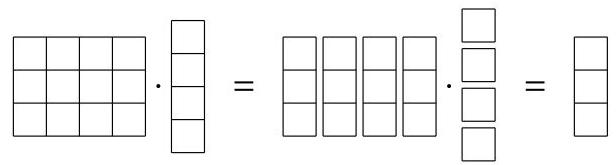
\includegraphics[width=0.5\textwidth]{images/ch06-fig07.jpg}}}
\end{equation}

设 \(B \in  {\mathbb{R}}^{k \times  n}\) 和 \(B = \left\lbrack  {{B}_{1}\cdots {B}_{n}}\right\rbrack\)。\({AB}\) 的第 \(j\) 列\(A{B}_{j}\) 是矩阵\(A\) 的各列的线性组合，其中系数由\({B}_{j}\)的各个分量给出。我们可以如下直观理解 \({AB}\) 的列(对于 \(n = 2\) ):
\begin{equation*}
\vcenter{\hbox{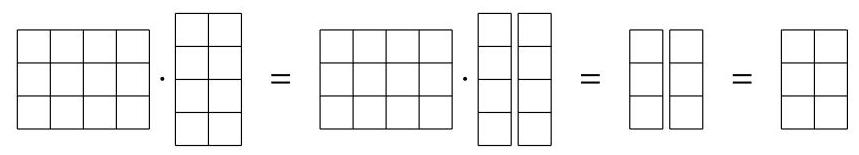
\includegraphics[width=0.65\textwidth]{images/ch06-fig08.jpg}}}
\end{equation*}

对 \({AB}\) 的第二种理解方式相同，但使用行。设 \(y \in  {\mathbb{R}}^{k}\) ，使得 \({y}^{\top }B\) 是 \({\mathbb{R}}^{1 \times  n}\) 中的一个行向量，它表示为 \(B\) 的行 \({b}_{1}^{\top },\ldots ,{b}_{k}^{\top }\) 的线性组合 \({y}_{1}{b}_{1}^{\top } + \cdots  + {y}_{k}{b}_{k}^{\top }\) (我们可以写成 \({B}^{\top } = \left\lbrack  {{b}_{1}\cdots {b}_{k}}\right\rbrack\) )，

\begin{equation}\label{eq:6.5}
\vcenter{\hbox{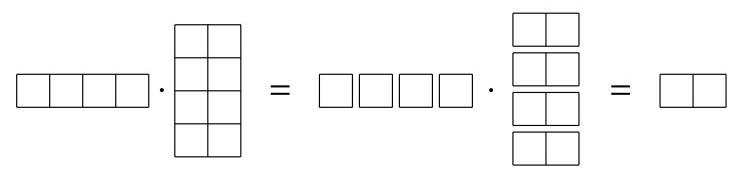
\includegraphics[width=0.6\textwidth]{images/ch06-fig09.jpg}}}
\end{equation}

设 \({A}^{\top } = \left\lbrack  {{a}_{1}\cdots {a}_{m}}\right\rbrack\) 。那么 \({AB}\) 的第 \(i\) 行是以 \(A\) 的第 \(i\) 行 \({a}_{i}^{\top }\) 的分量为系数的 \(B\) 的行的线性组合 \({a}_{i}^{\top }B\) :
\begin{equation*}
\vcenter{\hbox{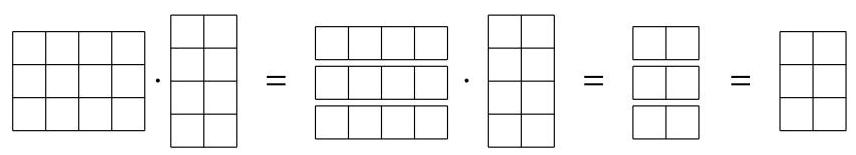
\includegraphics[width=0.65\textwidth]{images/ch06-fig10.jpg}}}
\end{equation*}

熟悉这些操作是很有用的。最常见的是矩阵与列向量右乘，如式\eqref{eq:6.4}所示；或者矩阵与行向量左乘，如式\eqref{eq:6.5}所示。

混合策略是参与者的一种随机策略。它被定义为该参与者纯策略集上的一种彩票(概率分布)。这是一种“主动随机化”玩法，参与者根据概率选择每种纯策略。当另一位参与者考虑对这种混合策略的最优反应时，假定她知道概率但不知道随机选择的结果，并根据由此产生的期望效用来做出决策。

纯策略被视为一种特殊的混合策略，它以概率1选择该纯策略(就像确定性结果被视为以概率1发生的“随机”结果一样)。

混合策略由它分配给参与者纯策略的概率决定。对于参与者I，混合策略 \(x\) 因此由它分配给参与者I的纯策略 \(1,2,\ldots ,m\) 的 \(m\) 维概率组合 \({x}_{1},{x}_{2},\ldots ,{x}_{m}\) 确定，我们将其写为(列)向量 \(x \in  {\mathbb{R}}^{m}\)。类似地，参与者II的混合策略 \(y\) 是纯策略 \(j = 1,\ldots ,n\) 的 \(n\) 维概率元组 \({y}_{1},\ldots ,{y}_{n}\)，写为 \(y \in  {\mathbb{R}}^{n}\) 。

参与者I和参与者II的混合策略集分别用 \(X\) 和 \(Y\) 表示。混合策略 \(x\) 中的概率 \({x}_{i}\) 是非负的，且总和为1，我们可以将 \(1 \leq  i \leq  m\) 和 \({x}_{1} + \cdots  + {x}_{m} = 1\) 的条件 \({x}_{i} \geq  0\) 写为 \(x \geq  \mathbf{0}\) 和 \({\mathbf{1}}^{\top }x = 1\) ，在这种情况下 \(\mathbf{1} \in  {\mathbb{R}}^{m}\) 以匹配 \(x\) 的维度；当我们类似地将 \({y}_{1} + \cdots  + {y}_{n} = 1\) 写为 \({\mathbf{1}}^{\top }y = 1\) 时，则 \(\mathbf{1} \in  {\mathbb{R}}^{n}\) 。即，
\begin{equation} \label{eq:6.6}
X = \left\{ x \in \mathbb{R}^{m} \;\middle|\; x \geq \mathbf{0},\; \mathbf{1}^{\top}x = 1 \right\}, \quad
Y = \left\{ y \in \mathbb{R}^{n} \;\middle|\; y \geq \mathbf{0},\; \mathbf{1}^{\top}y = 1 \right\} .
\end{equation}

对于 \(x \in  X\) 和 \(y \in  Y\) ，参与者 \(\mathrm{I}\) 的期望效用是 \({x}^{\top }{Ay}\) ，参与者II的期望效用是 \({x}^{\top }{By}\) 。最好将 \({x}^{\top }{Ay}\) 看作 \({x}^{\top }\left( {Ay}\right)\) ，即 \(x\) 与 \({Ay}\) 的标量积。对于每一行 \(i\) ， \({Ay}\) 中第 \(i\) 行的元素是 \({\left( Ay\right) }_{i}\) ，由下式给出
\begin{equation} \label{eq:6.7}
{\left( Ay\right) }_{i} = \mathop{\sum }\limits_{{j = 1}}^{n}{a}_{ij}{y}_{j}, \quad (1 \leq  i \leq  m).
\end{equation}


即， \({\left( Ay\right) }_{i}\) 是参与者 \(I\) 选择第 \(i\) 行时的期望效用。因此， \({x}^{\top }{Ay}\) 是当参与者使用 \(x\) 和 \(y\) 时参与者I的期望效用，因为
\begin{equation} \label{eq:6.8}
{x}^{\top }\left( {Ay}\right)  = \mathop{\sum }\limits_{{i = 1}}^{m}{x}_{i}{\left( Ay\right) }_{i} = \mathop{\sum }\limits_{{i = 1}}^{m}{x}_{i}\mathop{\sum }\limits_{{j = 1}}^{n}{a}_{ij}{y}_{j} = \mathop{\sum }\limits_{{i = 1}}^{m}\mathop{\sum }\limits_{{j = 1}}^{n}{x}_{i}{a}_{ij}{y}_{j}.
\end{equation}


由于参与者独立地选择他们的纯策略 \(i\) 和 \(j\)，他们选择纯策略对$(i, j)$的概率是这些概率的乘积 \({x}_{i}{y}_{j}\)，这就是式\eqref{eq:6.8}中收益 \({a}_{ij}\) 的系数。

类似地， \({x}^{\top }{By}\) 是当参与者使用混合策略 \(x\) 和 \(y\) 时参与者 II 的期望效用。在这里，最好将其理解为 \(\left( {{x}^{\top }B}\right) y\) 。行向量 \({x}^{\top }B\) 是参与者 II 对于她的列 \(j\) 的期望效用 \({\left( {x}^{\top }B\right) }_{j}\) 的向量。与列概率 \({y}_{j}\) 相乘后，所有列 \(j\) 的总和就是参与者 II 的期望效用，类似于式\eqref{eq:6.8}，其由下式给出

\[
\left( {{x}^{\top }B}\right) y = \mathop{\sum }\limits_{{j = 1}}^{n}{\left( {x}^{\top }B\right) }_{j}{y}_{j} = \mathop{\sum }\limits_{{j = 1}}^{n}\left( {\mathop{\sum }\limits_{{i = 1}}^{m}{x}_{i}{b}_{ij}}\right) {y}_{j} = \mathop{\sum }\limits_{{j = 1}}^{n}\mathop{\sum }\limits_{{i = 1}}^{m}{x}_{i}{b}_{ij}{y}_{j}.
\]

\section{最优反应条件}  \label{sec6.4}

混合策略均衡是一种混合策略组合，使得没有参与者可以通过单方面改变自己的策略来提高其期望效用。在两人博弈中，均衡是一对混合策略 $(x, y)$，使得 \(x\) 是对 \(y\) 的最优反应，反之亦然。要判断 \(x\) 是否是所有可能的混合策略中对 \(y\) 的最优反应，即 \(x\) 是否能使 \({x}^{\top }{Ay}\) 对于 \(X\) 中的所有 \(x\) 都达到最大，似乎并不容易，因为 \(X\) 是一个无限集。然而，下面这个被称为最优反应条件的命题展示了如何识别这一点。这个命题并不难但很重要。我们随后会讨论它。

\begin{proposition}[两人博弈的最优反应条件] \label{prop:6.1}
考虑一个 \(m \times  n\) 双矩阵博弈 $(A, B)$ 以及混合策略 \(x \in  X\) 和 \(y \in  Y\)。设
\begin{equation} \label{eq:6.9}
u = \max \left\{  {{\left( Ay\right) }_{i} \mid  1 \leq  i \leq  m}\right\}  ,\;v = \max \left\{  {{\left( {x}^{\top }B\right) }_{j} \mid  1 \leq  j \leq  n}\right\}.
\end{equation}
那么
\begin{equation} \label{eq:6.10}
\left( {\forall \bar{x} \in  X ~:~ {x}^{\top }{Ay} \geq  {\bar{x}}^{\top }{Ay}}\right) \; \Leftrightarrow  \;{x}^{\top }{Ay} = u,
\end{equation}
即， \(x\) 是对 \(y\) 的最优反应，当且仅当 \({x}^{\top }{Ay} = u\)。这等价于
\begin{equation} \label{eq:6.11}
{x}_{i} > 0 \Rightarrow  {\left( Ay\right) }_{i} = u \quad \left( {1 \leq  i \leq  m}\right).
\end{equation}

类似地， \(y\) 是对 \(x\) 的最优反应，当且仅当 \({x}^{\top }{By} = v\)。这等价于
\begin{equation} \label{eq:6.12}
{y}_{j} > 0 \Rightarrow  {\left( {x}^{\top }B\right) }_{j} = v\;\left( {1 \leq  j \leq  n}\right) .
\end{equation}
\end{proposition}

\begin{proof}
回顾 \({\left( Ay\right) }_{i}\) 是 \({Ay}\) 的第 \(i\) 个分量，如式~\eqref{eq:6.7}所示，它是参与者 I 选择第 \(i\) 行时的期望效用。参与者 \(\mathrm{I}\) 的纯策略的这些期望效用的最大值是 \(u\) 。那么
\begin{equation} \label{eq:6.13}
\begin{aligned}[b] % 使用 [b] 确保编号对齐最后一行
x^{\top}Ay
&= \sum_{i=1}^{m} x_i (Ay)_i  
= \sum_{i=1}^{m} x_i \bigl( u - (u - (Ay)_i ) \bigr) \\
&= \sum_{i=1}^{m} x_i u - \sum_{i=1}^{m} x_i \bigl( u - (Ay)_i \bigr) \\
&= u - \sum_{i=1}^{m} x_i \bigl( u - (Ay)_i \bigr).
\end{aligned}
\end{equation}


因为对于任何行 \(i\) 都有 \({x}_{i} \geq  0\) 和 \(u - {\left( Ay\right) }_{i} \geq  0\)，我们有 \(\mathop{\sum }\limits_{{i = 1}}^{m}{x}_{i}\left( {u - {\left( Ay\right) }_{i}}\right)  \geq  0\)，因此 \({x}^{\top }{Ay} \leq  u\)。期望效用 \({x}^{\top }{Ay}\) 达到最大值 \(u\) 当且仅当 \(\mathop{\sum }\limits_{{i = 1}}^{m}{x}_{i}\left( {u - {\left( Ay\right) }_{i}}\right)  = 0\) ，即如果 \({x}_{i} > 0\) 意味着 \({\left( Ay\right) }_{i} = u\)，这就证明了 式~\eqref{eq:6.11}。条件\eqref{eq:6.12}的证明类似。

我们用向量符号重复这个论证。首先，两个非负向量的标量积是非负的:对于 \(x,w \in  {\mathbb{R}}^{m}\) ，
\begin{equation} \label{eq:6.14}
x \geq  \mathbf{0},\;w \geq  \mathbf{0}\; \Rightarrow  \;{x}^{\top }w \geq  0.
\end{equation}

此外，式~\eqref{eq:6.9}意味着 \(\mathbf{1}u \geq  {Ay}\) ，即 \(w = \mathbf{1}u - {Ay} \geq  \mathbf{0}\) 。因此，
\begin{equation} \label{eq:6.15}
\begin{aligned}[b] % 使用 [b] 确保编号对齐最后一行
{x}^{\top }{Ay} &= {x}^{\top }\left( {\mathbf{1}u - \left( {\mathbf{1}u - {Ay}}\right) }\right)  = {x}^{\top }\mathbf{1}u - {x}^{\top }\left( {\mathbf{1}u - {Ay}}\right) \\
& = u - {x}^{\top }\left( {\mathbf{1}u - {Ay}}\right) \; \leq  u
\end{aligned}
\end{equation}

(注意 \({x}^{\top }\mathbf{1}u = \left( {{x}^{\top }\mathbf{1}}\right) u = 1 \cdot  u = u\) ，这显示了始终使用矩阵乘积的优势)。其次，式~\eqref{eq:6.14}可以扩展到
\begin{equation*}
x \geq  \mathbf{0},\;w \geq  \mathbf{0}\; \Rightarrow  \;\left( {{x}^{\top }w = 0\; \Leftrightarrow  \;{x}_{i}{w}_{i} = 0 \text{, 对于 }1 \leq  i \leq  m}\right)
\end{equation*}

因此，当且仅当对于 \(1 \leq  i \leq  m\) 有 \({x}_{i} = 0\) 或 \(u = {\left( Ay\right) }_{i}\) 时，式~\eqref{eq:6.15}中的 \({x}^{\top }{Ay} = u\) 成立，这与式~\eqref{eq:6.11}表述相同。
\end{proof}

如果混合策略 \(x\) 在 \(X\) 中的所有混合策略里，能为参与者 I 带来最大期望效用 \({x}^{\top }{Ay}\) ，如 式~\eqref{eq:6.10}左侧表述的那样，那么 \(x\) 就是对 \(y\) 的最优反应。相比之下，式~\eqref{eq:6.9}中的收益 \(u\) 是参与者 I 在所有纯策略 \(i\) 中的最大期望效用 \({\left( Ay\right) }_{i}\) 。根据式~\eqref{eq:6.10}，这些收益是相同的，所以参与者无法通过混合策略来提高其收益。这是符合直觉的，因为混合策略会如 式~\eqref{eq:6.8}那样，以概率 \({x}_{i}\) 为权重，对期望效用 \({\left( Ay\right) }_{i}\) 进行加权平均 \({x}^{\top }\left( {Ay}\right)\)。

此外，式~\eqref{eq:6.11}表明，当且仅当 \(x\) 仅以正概率 \({x}_{i}\) 选择纯最优反应时， \(x\) 才是对 \(y\) 的最优反应。判断一个纯策略是否为最优反应的条件很容易验证，因为只需要计算 \(i = 1,\ldots ,m\) 的 \(m\) 个期望效用 \({\left( Ay\right) }_{i}\) 即可。例如，如果参与者 I 有三个纯策略 \(\left( {m = 3}\right)\)，且式~\eqref{eq:6.7}中的期望效用分别为 \({\left( Ay\right) }_{1} = 4,{\left( Ay\right) }_{2} = 4\) 和 \({\left( Ay\right) }_{3} = 3\)，那么只有前两个策略是纯最优反应。如果这些期望效用分别为 3、5 和 3，那么只有第二个策略是最优反应。显然，至少存在一个纯最优反应，因为式~\eqref{eq:6.11}中的数字 \({\left( Ay\right) }_{i}\) 至少会在一个 \(i\) 处取得最大值 \(u\)。

最优反应条件是寻找混合策略均衡的核心工具，我们在此通过一个例子来进行说明；相关方法将在第\ref{sec6.6}节介绍。考虑以下 \(2 \times  3\) 博弈 $(A, B)$，我们已经标记出了最优反应收益，并给出了两个收益矩阵(由表格确定):
\begin{equation}   \label{eq:6.16}
A = \left( \begin{array}{lll} 0 & 4 & 0 \\  2 & 2 & 1 \end{array}\right) ,\;B = \left( \begin{array}{lll} 3 & 0 & 2 \\  1 & 6 & 4 \end{array}\right) .
\end{equation}

\begin{center}
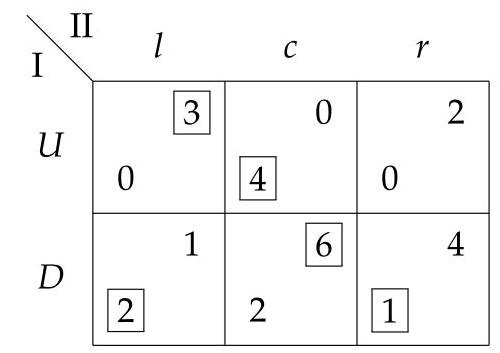
\includegraphics[width=0.4\textwidth]{images/ch06-fig11.jpg}
\end{center}
\hspace*{3em} 

这个博弈不存在纯策略均衡。对于任何纯策略，其唯一的最优反应是另一个参与者的纯策略，这不会导致均衡，因此两个参与者都必须采用非纯的混合策略。我们尝试寻找一个混合策略纳什均衡 $(x, y)$，其中 \(x = {\left( {x}_{1},{x}_{2}\right) }^{\top }\) 且 \(y = {\left( {y}_{1},{y}_{2},{y}_{3}\right) }^{\top }\)。(为了简洁，从现在起，在写具体向量时，我们将省略转置符号，例如只写 \(x = \left( {{x}_{1},{x}_{2}}\right)\)。)

由于参与者 I 只有两个纯策略，这两个策略都必须以正概率被采用，即 \({x}_{1} > 0\) 且 \({x}_{2} > 0\)。根据最优反应条件\eqref{eq:6.11}，参与者 I 必须对他的两行策略无差异，即
\begin{equation}   \label{eq:6.17}
{\left( Ay\right) }_{1} = {\left( Ay\right) }_{2} = u,\;4{y}_{2} = 2{y}_{1} + 2{y}_{2} + {y}_{3} = u,\;2{y}_{2} = 2{y}_{1} + {y}_{3}.
\end{equation} 

我们已经看到，当 \(y\) 是纯策略时，这无法实现，因此我们现在考虑在 \(y\) 下以正概率采用的任意一对策略。首先假设这些策略是前两列，即 \({y}_{1} > 0\) 、 \({y}_{2} > 0\) 和 \({y}_{3} = 0\)。那么，\eqref{eq:6.17}(以及 \({y}_{1} + {y}_{2} = 1\) )的唯一解是 \({y}_{1} = {y}_{2} = \frac{1}{2}\) ，其中 \(u = 2\)。继而，根据\eqref{eq:6.12}，参与者 II 必须对她的前两列无差异，即
\begin{equation}   \label{eq:6.18}
{\left( {x}^{\top }B\right) }_{1} = {\left( {x}^{\top }B\right) }_{2} = v,\;3{x}_{1} + {x}_{2} = 6{x}_{2},\;3{x}_{1} = 5{x}_{2}.
\end{equation} 

其唯一解为 \({x}_{1} = \frac{5}{8},{x}_{2} = \frac{3}{8}\) 和 \({\left( {x}^{\top }B\right) }_{1} = {\left( {x}^{\top }B\right) }_{2} = \frac{18}{8} = \frac{9}{4}\)。然而，我们还必须确保 \(\frac{9}{4}\) 是参与者 II 的最优反应收益，在 \(2 \times  2\) 博弈中这一考虑并非必要，在这类博弈中，只要两个参与者对他们的两种策略无差异即可。这里我们有 \({\left( {x}^{\top }B\right) }_{3} = \frac{22}{8} = \frac{11}{4} > \frac{9}{4}\)。也就是说，尽管参与者 II 对她的前两列无差异，这是因为 \({y}_{1} > 0\) 和 \({y}_{2} > 0\) 所必需的，但根据\eqref{eq:6.12}的要求，这些并非针对 \(x = \left( {\frac{5}{8},\frac{3}{8}}\right)\) 的纯最优反应。因此，不存在参与者 \(\mathrm{L}\) 采用她的前两列的混合策略纳什均衡。

接下来，假设参与者 II 选择她的第一列和第三列，其中 \({y}_{1} > 0,{y}_{2} = 0\) 和 \({y}_{3} > 0\)。然而，此时，式\eqref{eq:6.17}中的右侧方程表明 \(0 = 2{y}_{1} + {y}_{3}\)，这是不可能的。直观地说，当参与者 II 在式\eqref{eq:6.16}中仅采用第一列和第三列时，那么底行 \(D\) 是唯一的最优反应，并且无法使参与者 I 无差异。

这就只剩下最后一种可能性，即 \({y}_{1} = 0\) 、 \({y}_{2} > 0\) 和 \({y}_{3} > 0\)，此时，式\eqref{eq:6.17}变为 \(2{y}_{2} = {y}_{3}\)。因此 \({y}_{2} = \frac{1}{3},{y}_{3} = \frac{2}{3}\)。与式\eqref{eq:6.18}类似，我们现在需要
\begin{equation}   \label{eq:6.19}
{\left( {x}^{\top }B\right) }_{2} = {\left( {x}^{\top }B\right) }_{3} = v,\;6{x}_{2} = 2{x}_{1} + 4{x}_{2},\;2{x}_{1} = 2{x}_{2}
\end{equation} 

其唯一解为 \({x}_{1} = {x}_{2} = \frac{1}{2}\)，其中 \({\left( {x}^{\top }B\right) }_{2} = {\left( {x}^{\top }B\right) }_{3} = v = 3\)，由于 \({\left( {x}^{\top }B\right) }_{1} = 2 < 3\)， \(v\) 确实是预期列收益的最大值。我们已经找到了混合策略纳什均衡 \(x = \left( {\frac{1}{2},\frac{1}{2}}\right), y = \left( {0,\frac{1}{3},\frac{2}{3}}\right)\)。不存在参与者 II 以正概率选择所有三列的均衡，因为这意味着列无差异条件式\eqref{eq:6.18}和式\eqref{eq:6.19}，而它们的解 \(x\) 相互矛盾。因此，混合策略纳什均衡是唯一的。

\(\Rightarrow\) 练习~\ref{exer:6.2} 要求你找出一个 \(3 \times  2\) 博弈的所有混合策略纳什均衡，这可以用类似的方法完成，并能说明最优反应条件。它还为我们在第\ref{sec6.6}节中开发的寻找混合策略纳什均衡的方法提供了动机。

最优反应条件同样适用于有两个以上参与者的博弈，我们将在本节的剩余部分对此进行解释。在定义3.1中，我们为一个 \(N\) 参与者博弈定义了常用符号以及最优反应和均衡的概念。以下定义给出了它的混合扩展。对于参与者 \(i\) 的有限策略集 \({S}_{i}\)，根据定义5.1，我们用 \(\Delta \left( {S}_{i}\right)\) 表示 \({S}_{i}\) 上的混合策略集。

\begin{definition}[混合扩展]  \label{def:6.2}
考虑一个策略形式的 \(N\) 参与者博弈，其中参与者 \(i = 1,\ldots ,N\) 的有限策略集为 \({S}_{i}\) ，对于 \(S = {S}_{1} \times  \cdots  \times  {S}_{N}\) 中的每个策略组合 \(s = \left( {{s}_{1},\ldots ,{s}_{N}}\right)\) ，其收益为 \({u}_{i}\left( s\right)\) 。设 \({X}_{i} = \Delta \left( {S}_{i}\right)\) 为参与者 \(i\) 的混合策略 \({\sigma }_{i}\) 的集合，其中 \({\sigma }_{i}\left( {s}_{i}\right)\) 是 \({\sigma }_{i}\) 选择纯策略 \({s}_{i} \in  {S}_{i}\) 的概率。(如果对于某个 \({s}_{i}\) 有 \({\sigma }_{i}\left( {s}_{i}\right)  = 1\) ，则 \({\sigma }_{i}\) 被视为与纯策略 \({s}_{i}\) 相同。)那么，该博弈的混合扩展是一个策略形式的 \(N\) 参与者博弈，其(无限)策略集为 \({X}_{1},\ldots ,{X}_{N}\) ，对于所有 \(N\) 个参与者，在混合策略组合 \(\sigma  = \left( {{\sigma }_{1},\ldots ,{\sigma }_{N}}\right)\) 下，参与者 \(i\) 获得期望效用：

\[
{U}_{i}\left( \sigma \right)  = \mathop{\sum }\limits_{{s \in  S}}{u}_{i}\left( s\right) \mathop{\prod }\limits_{{k = 1}}^{N}{\sigma }_{k}\left( {s}_{k}\right) .
\]

混合扩展的一个均衡(或纳什均衡) \(\sigma\) 被称为原博弈的混合策略纳什均衡。
\end{definition}

以下命题将最优反应条件扩展到了一个 \(N\) 参与者博弈中。与两个参与者的情况一样，它使我们能够通过“参与者的混合策略仅以正概率选择纯最优反应”这一条件来验证一个混合策略组合是否为均衡。

\begin{proposition}[最优反应条件， \(N\) 个参与者] \label{prop:6.3}
考虑一个 \(N\) 参与者博弈的混合扩展，采用定义\ref{def:6.2}中的符号。设 \({\sigma }_{i} \in  {X}_{i}\) 为参与者 \(i\) 的混合策略，设 \({\sigma }_{-i}\) 为其他 \(N - 1\) 个参与者的混合策略的部分组合，并且设
\[
{v}_{i} = \max \left\{  {{U}_{i}\left( {{s}_{i},{\sigma }_{-i}}\right)  \mid  {s}_{i} \in  {S}_{i}}\right\}
\]

为参与者 \(i\) 的纯策略 \({s}_{i}\) 针对 \({\sigma }_{-i}\) 所能获得的最大期望效用。那么，当且仅当
\[
{\sigma }_{i}\left( {s}_{i}\right)  > 0 \Rightarrow  {U}_{i}\left( {{s}_{i},{\sigma }_{-i}}\right)  = {v}_{i}\;\left( {{s}_{i} \in  {S}_{i}}\right),
\]
即，如果 \({\sigma }_{i}\) 仅以正概率选择针对 \({\sigma }_{i}\) 的纯策略最优反应 \({s}_{i}\)。
\end{proposition}

\begin{proof}
证明过程与命题\ref{prop:6.1}的证明过程类似，只是将\eqref{eq:6.11}中的行 \(i\) (其中 \(i\) 表示一个纯策略)替换为纯策略 \({s}_{i}\) (其中 \(i\) 表示一个参与者)，并将 \({x}_{i}\) 替换为概率 \({\sigma }_{i}\left( {s}_{i}\right)\)。关键条件是，参与者 \(i\) 的期望效用关于其混合策略概率 \({\sigma }_{i}\left( {s}_{i}\right)\) 是线性的，因为对于一个混合策略组合 \(\sigma\)，
\begin{equation} \label{eq:6.20}
\begin{aligned}[b]
U_{i}(\sigma) 
&= U_{i}(\sigma_{i}, \sigma_{-i}) = \sum_{s \in S} u_{i}(s) \prod_{k=1}^{N} \sigma_{k}(s_{k}) \\
&= \sum_{s_{i} \in S_{i}} \sum_{s_{-i} \in S_{-i}} u_{i}(s_{i}, s_{-i}) \prod_{k=1}^{N} \sigma_{k}(s_{k}) \\
&= \sum_{s_{i} \in S_{i}} \left( \sum_{s_{-i} \in S_{-i}} u_{i}(s_{i}, s_{-i}) \prod_{k \neq i} \sigma_{k}(s_{k}) \right) \sigma_{i}(s_{i}) \\
&= \sum_{s_{i} \in S_{i}} U_{i}(s_{i}, \sigma_{-i}) \sigma_{i}(s_{i}).
\end{aligned}
\end{equation}

也就是说，期望效用 \({U}_{i}\left( \sigma \right)  = {U}_{i}\left( {{\sigma }_{i},{\sigma }_{-i}}\right)\) 恰好是以概率 \({\sigma }_{i}\left( {s}_{i}\right)\) 对“行” \({s}_{i} \in  {S}_{i}\) 的期望效用 \({U}_{i}\left( {{s}_{i},{\sigma }_{-i}}\right)\) 取期望，这里将参与者 \(i\) 视为行参与者。特别地，如果 \(N = 2\) 且 \(i\) 是参与者 1，那么 \({\sigma }_{-i}\) 是参与者 2 的混合策略 \(y\) ，而 \({U}_{i}\left( {{s}_{i},{\sigma }_{-i}}\right)\) 是行 \({s}_{i}\) 的期望效用 \({\left( Ay\right) }_{{s}_{i}}\)。用 \({\sigma }_{i}\) 代替 \(x\)， 用 \({v}_{i}\) 代替 \(u\) 后，\eqref{eq:6.13}中的证明与之前相同。
\end{proof}

{\(\Rightarrow\) 练习~\ref{exer:6.3} 是关于一个有三个参与者的博弈。}

我们继续关注两人博弈，部分原因是其符号表示更简单。更重要的是，对于两个参与者，最优反应条件比较的是期望效用(例如，对于行参与者的行 \(i\) 的 \({\left( Ay\right) }_{i}\) )，这些期望效用线性依赖于另一个参与者的混合策略概率 \({y}_{j}\) 。相比之下，\eqref{eq:6.20}中对于 \(N\) 个参与者且 \(N > 2\) 的相应表达式 \({U}_{i}\left( {{s}_{i},{\sigma }_{-i}}\right)\) 关于其他参与者的混合策略概率是非线性的，这使得在一般的 \(N\) 人博弈中找到混合策略纳什均衡变得困难得多。

\section{混合策略纳什均衡的存在性}   \label{sec6.5}

本节给出约翰·纳什(1951 年)关于混合策略纳什均衡存在性的原始证明。该证明表明，任意有限博弈都至少存在一个混合策略纳什均衡。证明过程中使用了布劳威尔不动点定理（见定理 \ref{theo:6.4}），该定理适用于紧凸集上的连续函数。\({\mathbb{R}}^{d}\) 的一个子集如果是闭集且有界，则它是紧的。

\({\mathbb{R}}^{d}\) 的一个子集 \(C\) 是凸集，如果它包含连接任意两点 \(x\) 和 \(y\) 的线段。如图 5.4 和 (5.45) 所述，\(C\) 是凸集当且仅当对于所有 \(x,y \in  C\) 和 \(\lambda  \in  \left\lbrack  {0,1}\right\rbrack\) 也有 \(x\left( {1 - \lambda }\right)  + {y\lambda } \in  C\)。这里我们将列向量 \(x\) 和 \(y\) 与右侧的标量 \(\left( {1 - \lambda }\right)\) 和 \(\lambda\) 相乘，使其形式与式 \eqref{eq:6.3} 的矩阵乘积一致。对于 \(\lambda  \in  \left\lbrack  {0,1}\right\rbrack\)，我们称 \(x\left( {1 - \lambda }\right)  + {y\lambda }\) 是 \(x\) 和 \(y\) 的凸组合(它是连接 \(x\) 和 \(y\) 的线段上的任意一点)。一般地， \({\mathbb{R}}^{d}\) 中的点 \({z}_{1},{z}_{2},\ldots ,{z}_{n}\) 的凸组合是指形如 \({z}_{1}{\lambda }_{1} + {z}_{2}{\lambda }_{2} + \cdots  + {z}_{n}{\lambda }_{n}\)的线性组合，其中系数 \({\lambda }_{1},\ldots ,{\lambda }_{n}\) 非负且和为 1。

\begin{figure}[htbp] \label{fig:6.5}
  \centering
  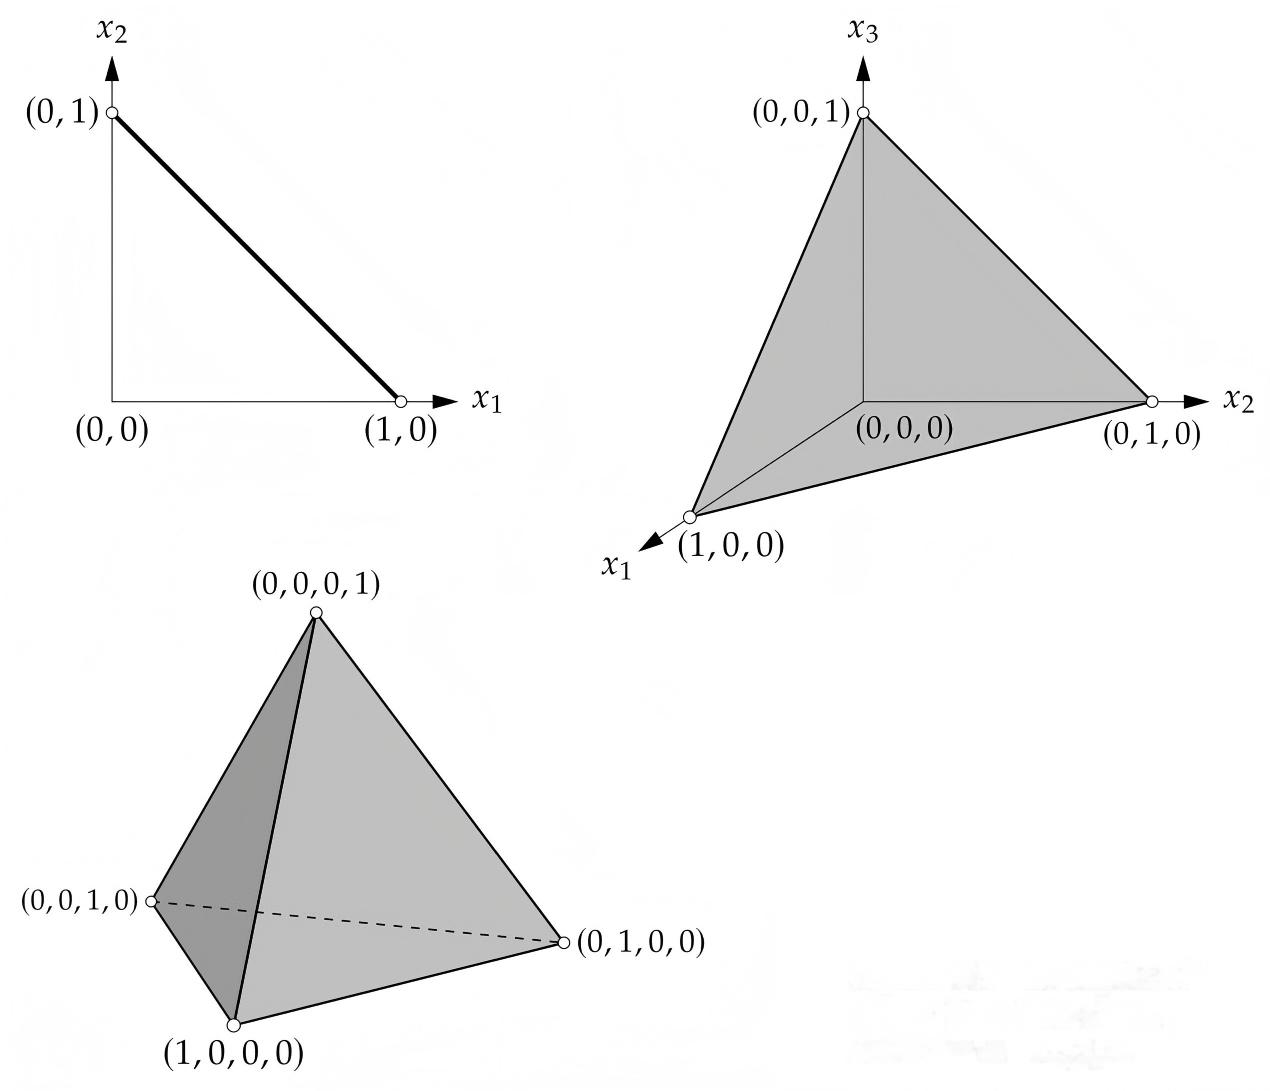
\includegraphics[width=1.0\textwidth]{images/ch06-fig12.jpg}
\caption{当 $m=2,3,4$ 时，玩家 I 的混合策略集合$X$的示例。}
\end{figure}


参与者的混合策略集是特殊的凸集。对于一个 \(m \times  n\) 博弈，参与者 I 和参与者 II 的混合策略集分别为\eqref{eq:6.6} 式中的 \(X\) 和 \(Y\)。 \({\mathbb{R}}^{m}\) 中的第 \(i\) 个单位向量 \({e}_{i}\) (其中 \(1 \leq  i \leq  m\) )定义为\({\left( 0,\ldots ,0,1,0,\ldots ,0\right) }^{\top }\)，其中第 \(i\) 个分量为 1，其他分量均为 0。这个向量属于 \(X\)，表示参与者 I 的纯策略 \(i\)。对于 \(X\) 中的任何混合策略 \(x = {\left( {x}_{1},\ldots ,{x}_{m}\right) }^{\top }\)，显然有 \(x = {e}_{1}{x}_{1} + {e}_{2}{x}_{2} + \cdots  + {e}_{n}{x}_{m}\)，即 \(x\) 表示为单位向量\({e}_{1},\ldots ,{e}_{m}\) 的凸组合，且对应的系数是混合策略的概率 \({x}_{1},\ldots ,{x}_{m}\) (因为这些概率是非负的且总和为 1)。类似地，任何混合策略 \(y \in  Y\) 是 \({\mathbb{R}}^{n}\) 中单位向量的凸组合，这些单位向量表示参与者 II 的纯策略。

图\ref{fig:6.5} 展示了当 \(m = 2,3,4\) 时混合策略集\(X\)的情形，其中 \(X\) 分别对应于线段、三角形和四面体。一般来说， \({\mathbb{R}}^{m}\) 中 \(m\) 个单位向量的凸包称为单位单纯形。容易看出， \(X\) 和 \(Y\) 以及它们的笛卡尔积 \(X \times  Y\) 都是凸集(见下面的\eqref{eq:6.23}式)。为了证明混合策略纳什均衡的存在性，我们将对集合 \(C = X \times  Y\) 上的适当连续函数 \(f : C \rightarrow  C\) 使用布劳威尔不动点定理。

\begin{theorem}[布劳威尔不动点定理] \label{theo:6.4}  %定理 6.4
设 \(C\) 是 \({\mathbb{R}}^{d}\) 的一个非空子集，它是凸集且是紧集，设 \(f\) 是从 \(C\) 到 \(C\) 的连续函数。那么， \(f\) 至少有一个不动点，即 \(C\) 中存在一点 \(z\)，使得 \(f\left( z\right)  = z\)。
\end{theorem}

\begin{figure}[htbp]  \label{fig:6.6}
  \centering
  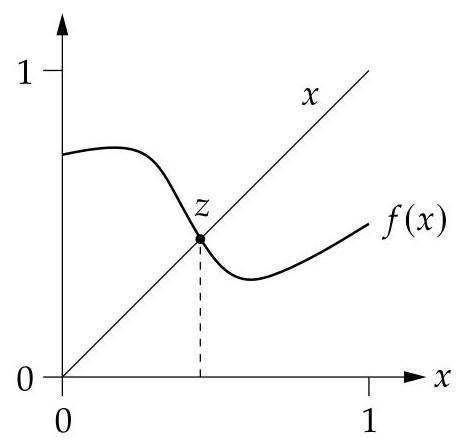
\includegraphics[width=0.3\textwidth]{images/ch06-fig13.jpg}
  \caption{区间 $C=[0,1]$ 情况下布劳威尔不动点定理的证明}
\end{figure}


图\ref{fig:6.6} 展示了定理\ref{theo:6.4} 在区间 \(C = \left\lbrack  {0,1}\right\rbrack\) 上的情形。如果连续函数 \(f : C \rightarrow  C\) 满足 \(f\left( 0\right)  = 0\)，那么 0 是 \(f\) 的一个不动点；类似地，如果 \(f\left( 1\right)  = 1\)，那么 1 是 \(f\) 的一个不动点。因此，我们可以假设 \(f\left( 0\right)  > 0\) 且 \(f\left( 1\right)  < 1\) 。那么，函数 \(f\) 的图至少与恒等函数 \(x \mapsto  x\) 的线相交一次，交点为 \(z\)，此时 \(f\left( z\right)  = z\)，这就是我们所需要的不动点。更正式地说，连续函数 \(x \mapsto  x - f\left( x\right)\) 在 \(x = 0\) 处为负，在 \(x = 1\) 处为正，根据介值定理，对于介于两者之间的值 \(z\) (其中 \(0 < z < 1\) )，该函数值为 0，即 \(z - f\left( z\right)  = 0\) 或 \(f\left( z\right)  = z\)。

以下简单示例表明，定理\ref{theo:6.4}中的假设条件是必要的。考虑由 \(f\left( x\right)  = x + 1\) 定义的函数 \(f : \mathbb{R} \rightarrow  \mathbb{R}\)。这显然是一个连续函数，并且所有实数的集合 \(\mathbb{R}\) 是闭集且凸集，但 \(f\) 没有不动点。此时，不动点定理的某些假设必定不成立；事实上，对于前述情形，因为集合 \(\mathbb{R}\) 是无界的，所以它不满足紧性。再考虑另一个函数 \(f : \left\lbrack  {0,1}\right\rbrack   \rightarrow  \left\lbrack  {0,1}\right\rbrack\)，由 \(f\left( x\right)  = {x}^{2}\) 给出，这个函数的不动点是0和1。如果我们将函数 \(f\left( x\right)  = {x}^{2}\) 定义在开区间(0,1)上，那么这个函数就不再有任何不动点。在这种情况下，缺失的条件是函数不是定义在闭集上，即定义域不满足紧集的要求。接下来，考虑定义在\(x \in  \{ 0,1\}\) 上的函数 \(f\left( x\right)  = 1 - x\) ，该函数的定义域只有两个元素，所以这是一个紧集。但是，这个函数没有不动点，因为它的定义域不是凸集。最后，考虑定义在 \(\left\lbrack  {0,1}\right\rbrack\) 上的函数：当 \(0 \leq  x \leq  \frac{1}{2}\) 时为 \(f\left( x\right)  = 1\) ，当 \(\frac{1}{2} < x \leq  1\) 时为 \(f\left( x\right)  = 0\) 。这个函数没有不动点，因为该函数不连续。这些示例说明了为什么定理\ref{theo:6.4}的假设条件是必要的。

定理\ref{theo:6.4}是拓扑学中的一个重要定理，对于一般维度 \(d\) 而言，其证明要困难得多。我们将在第7章给出完整的证明。

以下定理阐述了混合策略纳什均衡的存在性。我们使用布劳威尔不动点定理，按照纳什(1951)原始证明的思路来证明它。为简化符号，这里考虑两个参与者的情况。

\begin{theorem}[纳什，1951]  \label{theo:6.5}  %定理6.5
    每个有限博弈至少有一个混合策略纳什均衡。
\end{theorem}

\begin{proof}
    为简化符号，我们将给出 \(m \times  n\) 两人博弈$(A, B)$的证明。证明过程可以类似地推广到任意有限数量的参与者。设 \(X\) 和 \(Y\) 分别是参与者I和参与者II的混合策略集合，如式\eqref{eq:6.6}所示。设 \(C = X \times  Y\)，即集合 \(C\) 是参与者的混合策略集合的笛卡尔积；显然它是凸集且是紧集。

然后，我们要构建函数 \(f : C \rightarrow  C\) 将混合策略组 $(x, y)$ 映射到另一个混合策略组，即\(f\left( {x,y}\right)  = \left( {\bar{x},\bar{y}}\right)\)。直观地说，参与者 I 的混合策略概率 \({x}_{i}\) (同理，参与者 II 的 \({y}_{j}\))会变为 \({\bar{x}}_{i}\)，如果纯策略 \(i\) 的表现优于当前期望效用 \({x}^{\top }{Ay}\)，则 \({x}_{i}\) 会增加。如果纯策略 \(i\) 的表现较差，那么除非 \({x}_{i}\) 已经为零，否则 \({x}_{i}\) 会减小。在均衡状态下，\(x\) 是对 \(y\) 的最优反应，并且根据式\eqref{eq:6.10}，\({x}^{\top }{Ay} = u\)，其中 \(u\) 为纯策略最优反应的收益，同时所有次优纯策略的概率为零。这意味着混合策略 \(x\) 不会改变，即 \(\bar{x} = x\) 。类似地，如果 \(y\) 是对 \(x\) 的最优反应，那么 \(\bar{y} = y\)。因此，均衡性质等价于不动点性质 \(\left( {x,y}\right)  = \left( {\bar{x},\bar{y}}\right)  = f\left( {x,y}\right)\)。

为了定义如上所述的 \(f\) ，考虑以下函数 \(\chi  : X \times  Y \rightarrow\)  \({\mathbb{R}}^{m}\) 和 \(\psi  : X \times  Y \rightarrow  {\mathbb{R}}^{n}\)。对于参与者 I 的任意纯策略 \(i\)，令 \({\chi }_{i}\left( {x,y}\right)\) 为 \(\chi \left( {x,y}\right)\) 的第 \(i\) 个分量；对于参与者 II 的任意纯策略 \(j\) ，令 \({\psi }_{j}\left( {x,y}\right)\) 为 \(\psi \left( {x,y}\right)\) 的第 \(j\) 个分量。函数 \(\chi\) 和 \(\psi\) 定义如下
\begin{equation}
\label{eq:6.21}
\begin{aligned}
\chi_i(x,y)
&= \max \left\{ 0,\,(Ay)_i - x^{\top}Ay \right\},
\quad &(1 \le i \le m), \\
\psi_j(x,y)
&= \max \left\{ 0,\,(x^{\top}B)_j - x^{\top}By \right\},
\quad &(1 \le j \le n).
\end{aligned}
\end{equation}



回顾一下， \({\left( Ay\right) }_{i}\) 是参与者 I 使用纯策略 \(i\) 对抗 \(y\) 时的期望效用， \({\left( {x}^{\top }B\right) }_{j}\) 是参与者 II 使用纯策略 \(j\) 对抗 \(x\) 时的期望效用， \({x}^{\top }{Ay}\) 和 \({x}^{\top }{By}\) 分别是参与者 \(\mathrm{I}\) 和参与者 II 的期望效用。因此，如果纯策略 \(i\) 对抗 \(y\) 时的收益高于平均收益 \({x}^{\top }{Ay}\) ，则差值 \({\left( Ay\right) }_{i} - {x}^{\top }{Ay}\) 为正；如果收益相同，则差值为零；如果收益较低，则差值为负。\({\chi }_{i}\left( {x,y}\right)\) 就是这个差值，但如果差值为负，则该项被替换为零。\({\psi }_{j}\left( {x,y}\right)\) 的定义类似。因此， \(\chi \left( {x,y}\right)\) 是 \({\mathbb{R}}^{m}\) 中的非负向量， \(\psi \left( {x,y}\right)\) 是 \({\mathbb{R}}^{n}\) 中的非负向量。函数 \(\chi\) 和 \(\psi\) 是连续的。

现在，将向量组 $(x, y)$改变：将 \(x\) 替换为 \(x + \chi \left( {x,y}\right)\) 以得到 \(\bar{x}\)，将 \(y\) 替换为 \(y + \psi \left( {x,y}\right)\) 以得到 \(\bar{y}\)。两个向量的和都是非负的。然而，这些新向量通常不再是混合策略，因为它们的分量之和不一定是1。因此，通过以下连续函数 \(r\) 和 \(s\) 对它们进行“重新归一化”：对于非零非负向量 \(x \in  {\mathbb{R}}^{m}\) 和 \(y \in  {\mathbb{R}}^{n}\)，
\[
r\left( x\right)  = x\frac{1}{{\mathbf{1}}^{\top }x},\quad s\left( y\right)  = y\frac{1}{{\mathbf{1}}^{\top }y}.
\]

于是，\(r\left( x\right)  \in  X\)，因为 \({\mathbf{1}}^{\top }r\left( x\right)  = {\mathbf{1}}^{\top }x\frac{1}{{\mathbf{1}}^{\top }x} = 1\)。类似地，\(s\left( y\right)  \in  Y\)。我们定义函数 \(f : C \rightarrow  C\) 如下：
\[
f\left( {x,y}\right)  = \left( {r\left( {x + \chi \left( {x,y}\right) }\right) ,s\left( {y + \psi \left( {x,y}\right) }\right) }\right).
\]

我们断言
\begin{equation}
\label{eq:6.22}
\begin{aligned}
x &= r\!\left( x + \chi(x,y) \right)
\;\Longleftrightarrow\;
x \text{ 是 } y \text{ 的最优反应}, \\
y &= s\!\left( y + \psi(x,y) \right)
\;\Longleftrightarrow\;
y \text{ 是 } x \text{ 的最优反应}.
\end{aligned}
\end{equation}
这表明：$(x, y)$ 是 \(f\) 的一个不动点当且仅当 $(x, y) $是博弈$ (A, B) $的一个均衡。

根据对称性，只需证明 \eqref{eq:6.22}中的第一个等价关系。其中“ \(\Leftarrow\) ”很容易:如果 \(x\) 是对 \(y\) 的最优反应，那么最优反应条件\eqref{eq:6.10}意味着\eqref{eq:6.21}中的 \(\chi \left( {x,y}\right)  = \mathbf{0} \in  {\mathbb{R}}^{m}\)，因此 \(x = r\left( {x + \chi \left( {x,y}\right) }\right)\)。

反之，设 \(x = r\left( {x + \chi \left( {x,y}\right) }\right)\)。理论上，如果 \(\chi \left( {x,y}\right)  \neq  \mathbf{0}\) (使得 \(x\) 不是对 \(y\) 的最优反应)，由于用 \(r\) 进行重新归一化，那么\(x = r\left( {x + \chi \left( {x,y}\right) }\right)\)可能成立，例如如果 \(x = \left( {\frac{1}{3},\frac{1}{3},\frac{1}{3}}\right)\) 且 \(\chi \left( {x,y}\right)  = \left( {\frac{1}{5},\frac{1}{5},\frac{1}{5}}\right)\)。然而，这是不可能的。设
\begin{equation*}
\begin{aligned}
u
&= \max \left\{ (Ay)_i \mid 1 \le i \le m \right\}
 = (Ay)_{\ell}, \\
t
&= \min \left\{ (Ay)_i \mid 1 \le i \le m,\; x_i > 0 \right\}
 = (Ay)_k,
 \qquad \text{with } x_k > 0.
\end{aligned}
\end{equation*}


类似于\eqref{eq:6.13}，可得 \(t \leq  {x}^{\top }{Ay}\)，因此 \({\chi }_{k}\left( {x,y}\right)  = 0\)。如果 \(x\) 不是对 \(y\) 的最优反应，那么 \({x}^{\top }{Ay} < u\)，因此 \({\chi }_{\ell }\left( {x,y}\right)  > 0\) 且 \({\mathbf{1}}^{\top }\left( {x + \chi \left( {x,y}\right) }\right)  > 1\)，即 \(\frac{1}{{\mathbf{1}}^{\top }\left( {x + \chi \left( {x,y}\right) }\right) } < 1\)。因为 \({\chi }_{k}\left( {x,y}\right)  = 0\)，这意味着重新归一化后的向量 \(\bar{x} = r\left( {x + \chi \left( {x,y}\right) }\right)\) 在其正的第 \(k\) 个分量 \({\bar{x}}_{k} < {x}_{k}\) 上缩小，这与假设 \(\bar{x} = x\) 矛盾。这证明了\eqref{eq:6.22}中的“ \(\Rightarrow\) ”。

如所断言，因此不动点 $(x, y)$ 恰好是博弈的均衡，并且根据布劳威尔不动点定理\ref{theo:6.4}，该博弈至少存在一个均衡。
\end{proof}

我们将在第 7 章给出布劳威尔不动点定理的证明。
 
\section{小规模博弈中混合策略纳什均衡的求解}  \label{sec6.6}

如何找到两人策略型博弈的所有均衡呢？我们能比较容易的确定纯策略均衡，因为它们是收益表中两个收益都被框起来作为最优反应收益的单元格。我们现在论述如何使用命题\ref{prop:6.1}给出的最优反应条件来找到混合策略均衡。

我们首先考虑 \(2 \times  2\) 博弈。我们上面的第一个例子，即图\ref{fig:6.2}中的监管博弈，没有纯策略均衡。在那里，我们确定了一个参与者的混合策略概率，以便让另一个参与者在她的纯策略之间无差异，因为只有这样她才会在这些策略之间进行混合。这是命题\ref{prop:6.1}的一个推论:在均衡状态下，只有那些获得最大(因此相等)期望效用的纯策略才有可能以正概率被采用。

\begin{figure}[htbp]
  \centering
  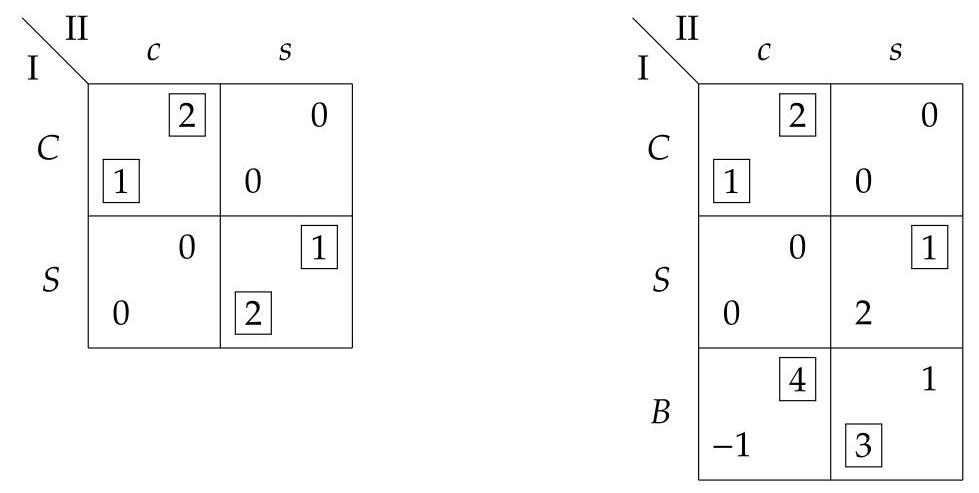
\includegraphics[width=0.7\textwidth]{images/ch06-fig14.jpg}
  \caption{性别战博弈（左）和一个 $3 \times 2$ 博弈（右），后者是参与者 I 增加了一个额外策略 $B$ 的相同博弈。}
  \label{fig:6.7}
\end{figure}


\begin{figure}[htbp]
  \centering
  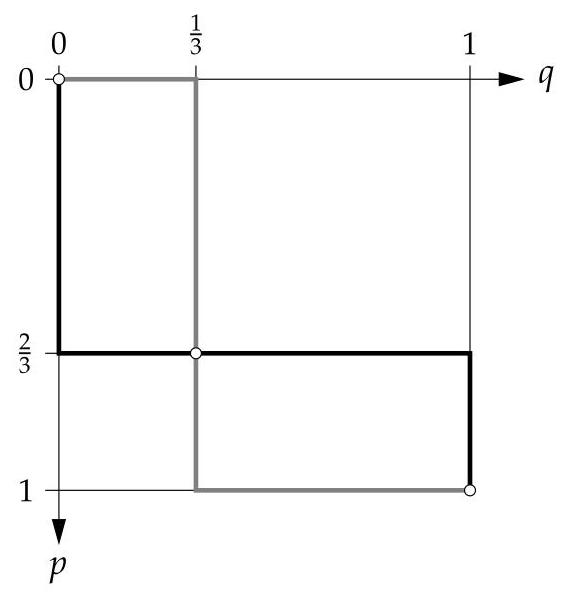
\includegraphics[width=0.4\textwidth]{images/ch06-fig15.jpg}
  \caption{性别战 $2 \times 2$ 博弈（图\ref{fig:6.7} 左侧）的最优反应混合策略 $(1-p,p)$（灰色）和 $(1-q,q)$（黑色）。该博弈有两个纯策略均衡 $\big((1,0),(1,0)\big)$ 和 $\big((0,1),(0,1)\big)$，以及一个混合策略纳什均衡 $\big((\frac{1}{3},\frac{2}{3}),(\frac{2}{3},\frac{1}{3})\big)$。}
  \label{fig:6.8}
\end{figure}


在具有纯策略均衡的 \(2 \times  2\) 博弈中，也可能存在混合策略均衡。例如，考虑图\ref{fig:6.7}左侧的性别战博弈。最优反应效用表明，该博弈存在纯策略均衡 $(C, c)$ 和 $(S, s)$。现在假设参与者I采用混合策略 \(x = \left( {1 - p,p}\right)\) ，参与者II采用混合策略 \(y = \left( {1 - q,q}\right)\) 。与图\ref{fig:6.4}中的监管博弈类似，图\ref{fig:6.8}展示了参与者针对对方混合策略的最优反应。例如，如果 \(p = \frac{1}{2}\) ，那么参与者II在列 \(c\) 的期望效用为1，在列 \(s\) 的期望效用为 \(\frac{1}{2}\) ，她的最优反应是 \(c\) ，即混合策略 (1,0)，其中 \(q = 0\) 。一般来说， \(c\) 和 \(s\) 的效用分别为 \(2\left( {1 - p}\right)\) 和 \(p\) ，因此如果 \(2\left( {1 - p}\right)  \geq  p\) 或者等价地 \(\frac{2}{3} \geq  p\) ，即 \(p \in  \left\lbrack  {0,\frac{2}{3}}\right\rbrack\) ，参与者II弱偏好 \(c\) 而非 \(s\) 。对于 \(p = \frac{2}{3}\) ，参与者II无差异，任何 \(q \in  \left\lbrack  {0,1}\right\rbrack\) 都定义了一个最优反应 $(1 - q, q)$。对于 \(p > \frac{2}{3}\) ，参与者II严格偏好 \(s\) 而非 \(c\) ，这定义了唯一的最优反应 (0,1)。类似地，参与者 \(\mathrm{I}\) 针对混合策略 (1 - q, q) 的最优反应混合策略 (1 - p, p) 为:当 \(q \in  \left\lbrack  {0,\frac{1}{3}}\right)\) 时为 \(p = 0\) ；当 \(q = \frac{1}{3}\) 时，任何 \(p \in  \left\lbrack  {0,1}\right\rbrack\) 均可；当 \(q \in  \left( {\frac{1}{3},1}\right\rbrack\) 时为 \(p = 1\) (快速验证的一个例子是 \(q = \frac{1}{2}\) ，此时策略 \(S\) 给参与者 \(\mathrm{I}\) 带来更高的期望效用)。除了纯策略均衡之外，这给出了混合策略纳什均衡 \(\left( {\left( {\frac{1}{3},\frac{2}{3}}\right) ,\left( {\frac{2}{3},\frac{1}{3}}\right) }\right)\) 。

总之，在 \(2 \times  2\) 博弈中寻找混合策略均衡的规则是让对方参与者无差异，因为只有在这种情况下，对方参与者才会采用混合策略。然后，两个对手策略的期望效用必须相等，由此得到的方程决定了参与者自身的概率。

通过观察效用矩阵，可以相对快速地看出性别战博弈中的混合策略概率:例如，参与者II对左列 \(c\) 的权重必须是右列 \(s\) 的两倍，因为当参与者II选择 \(c\) 时，参与者I的顶行 \(C\) 只能获得效用1，而当她选择 \(s\) 时，他的底行 \(S\) 能获得效用2，并且策略组合 (C, s) 和 (S, c) 的效用为零。因此，只有当参与者II分别以概率 \(\frac{2}{3}\) 和 \(\frac{1}{3}\) 混合 \(c\) 和 \(s\) 时，两行 \(C\) 和 \(S\) 才具有相同的期望效用。

\begin{figure}[htbp]
  \centering
  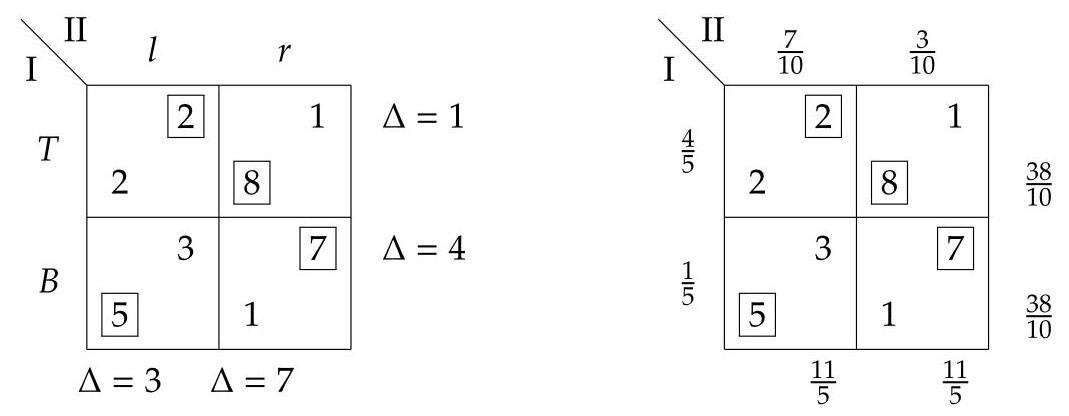
\includegraphics[width=0.8\textwidth]{images/ch06-fig16.jpg}
  \caption{用于在 $2 \times 2$ 博弈中寻找混合策略纳什均衡概率的“差分技巧”。左图展示了该博弈，以及每个纯策略下另一个参与者的收益差异。右图显示这些差异被分配到各自的另一个自身策略，并重新归一化为概率。分数 $\frac{11}{5}$ 和 $\frac{38}{10}$ 分别是参与者 II 和参与者 I 的期望效用相等的结果。}
  \label{fig:6.9}
\end{figure}


我们现在解释一种快速方法，即“差分技巧”，用于在一般的 \(2 \times  2\) 博弈中寻找混合策略纳什均衡的概率。考虑图\ref{fig:6.9}左侧的博弈。当参与者I选择 \(T\) 时， \(l\) 是最优反应；当参与者I选择 \(B\) 时， \(r\) 是最优反应。因此，必然存在一种方法来混合 \(T\) 和 \(B\) ，使得参与者II在 \(l\) 和 \(r\) 之间无差异。我们现在考虑两行中另一个参与者的收益差异 \(\Delta\) :当参与者 \(\mathrm{I}\) 选择 \(T\) 时，参与者II的两个收益之间的差异是 \(\Delta  = 2 - 1 = 1\) ；当参与者I选择 \(B\) 时，该差异的绝对值是 \(\Delta  = 7 - 3 = 4\) ，如博弈图旁边所示。(注意，当将这些差异视为 \(l\) 与 \(r\) 的收益之间的差异时，它们的符号相反，因为在面对 \(T\) 时， \(l\) 优于 \(r\) ，而在面对 \(B\) 时则相反；否则，参与者II将总是偏好相同的策略，并且无法使其无差异。)现在，收益差异 \(\Delta\) 被作为概率权重分配给行参与者的各自另一个策略，即 \(T\) 的权重为4(这是为 \(B\) 计算的 \(\Delta\) )， \(B\) 的权重为1(这是为 \(T\) 计算的 \(\Delta\) )。然后， \(T\) 和 \(B\) 的概率选择与这些权重成比例，因此必须将每个权重除以5(这是权重之和)以获得概率。这在图\ref{fig:6.9}的右侧展示。参与者II的期望效用也显示在那里，在底部， \(l\) 的期望效用由 \(\left( {4 \cdot  2 + 1 \cdot  3}\right) /5 = \frac{11}{5}\) 给出， \(r\) 的期望效用由 \(\left( {4 \cdot  1 + 1 \cdot  7}\right) /5 = \frac{11}{5}\) 给出，因此它们确实如所声称的那样相等。类似地，参与者I在列 \(l\) 和 \(r\) 中的两个收益差异分别为3和7，因此 \(l\) 和 \(r\) 的选择概率应分别与7和3成比例。使用得到的概率 \(\frac{7}{10}\) 和 \(\frac{3}{10}\) ，两行 \(T\) 和 \(B\) 获得相同的期望效用 \(\frac{38}{10}\) 。

\(\Rightarrow\) 练习~\ref{exer:6.4} 要求你证明这种“差分技巧”总是有效的。

接下来，我们考虑一方参与者有两种策略而另一方参与者有超过两种策略的博弈。图\ref{fig:6.7}右侧的 \(3 \times  2\) 博弈与性别战博弈类似，不同之处在于参与者I有一个额外的策略B。本质上，此类博弈可以通过考虑仅限制双方参与者使用两种策略而得到的 \(2 \times  2\) 博弈来进行分析，并检查由此得到的均衡是否适用于整个博弈。首先，原始性别战博弈的纯策略均衡$(C, c)$也是这个更大博弈的一个均衡，但$(S, s)$不是，因为 \(S\) 不再是对 \(s\) 的最优反应，因为 \(B\) 给参与者I带来了更高的收益。其次，考虑较小博弈的混合策略均衡，其中参与者I以概率 \(\frac{1}{3}\) 和 \(\frac{2}{3}\) 选择 \(C\) 和 \(S\) (以概率零选择 \(B\) )，从而使参与者II在 \(c\) 和 \(s\) 之间无差异。因此，参与者II的混合策略 \(\left( {\frac{2}{3},\frac{1}{3}}\right)\) 仍然是最优反应，在这种情况下， \(C\) 和 \(S\) 都给出相同的期望效用 \(\frac{2}{3}\) 。然而，这并不足以保证达到均衡，因为 \(C\) 和 \(S\) 必须是最优反应，即它们的收益必须至少与额外策略 \(B\) 的收益一样大。该收益为 \(\left( {-1}\right)  \cdot  \frac{2}{3} + 3 \cdot  \frac{1}{3} = \frac{1}{3}\) ，所以它确实不大于 \(C\) 和 \(S\) 的收益。换句话说，较小博弈的混合策略纳什均衡也是较大博弈的混合策略纳什均衡，由混合策略对 \(\left( {\left( {\frac{1}{3},\frac{2}{3},0}\right) ,\left( {\frac{2}{3},\frac{1}{3}}\right) }\right)\) 给出。

其他“受限”的 \(2 \times  2\) 博弈可通过让参与者I仅采用 \(C\) 和 \(B\) 策略，或者仅采用 \(S\) 和 \(B\) 策略来获得。在第一种情况下，差分技巧给出了参与者II的混合策略 \(\left( {\frac{3}{5},\frac{2}{5}}\right)\) (用于采用 \(c,s\) )，使得参与者I在 \(C\) 和 \(B\) 之间无差异，此时这两种策略的期望效用均为 \(\frac{3}{5}\) 。然而，第三种策略 \(S\) 的期望效用为 \(\frac{4}{5}\) ，这更高，因此 \(C\) 和 \(B\) 不是最优反应，这意味着我们无法得到一个参与者I仅以正概率采用 \(C\) 和 \(B\) 的均衡。参与者II没有混合采用 \(C\) 和 \(B\) 的均衡策略的另一个原因是，对于 \(C\) 和 \(B\) ，参与者II的最优反应始终是 \(c\) ，因此参与者I无法通过仅采用 \(C\) 和 \(B\) 使参与者II无差异。

最后，考虑将 \(S\) 和 \(B\) 作为参与者I在可能的均衡中混合采用的纯策略。通过差分技巧，这需要参与者I采用混合策略 \(\left( {0,\frac{3}{4},\frac{1}{4}}\right)\) (作为采用他的三个纯策略 \(C,S,B\) 的概率向量)，从而使参与者II在 \(c\) 和 \(s\) 之间无差异，且两种策略的收益均为1。然后，如果参与者II采用混合策略 \(\left( {\frac{1}{2},\frac{1}{2}}\right)\) (以使参与者I在 \(S\) 和 \(B\) 之间无差异)，则三行策略 \(C,S,B\) 的期望效用分别为 \(\frac{1}{2},1\) 和1，因此参与者I确实仅以正概率采用最优反应，这给出了该博弈的第三个均衡。

为什么图\ref{fig:6.7}中的 \(3 \times  2\) 博弈不存在参与者I在其三种纯策略之间进行混合的混合策略纳什均衡呢？原因在于参与者II只能使用单一概率(该概率决定了另一种纯策略的互补性概率)，这不足以满足两个方程，即 \(C\) 和 \(S\) 之间的无差异以及 \(S\) 和 \(B\) 之间的无差异(第三个无差异，即 \(C\) 和 \(B\) 之间的无差异会自动成立)。我们已经计算出了使得 \(C\) 和 \(S\) 具有相同期望效用所需的 \(c,s\) 的概率 \(\left( {\frac{2}{3},\frac{1}{3}}\right)\) ，而在此情况下，行 \(B\) 的效用不同，即为 \(\frac{1}{3}\) 。仅此一点就足以表明，不可能使参与者I在所有三种纯策略之间保持无差异，因此不存在参与者I在所有这些策略之间进行混合的均衡。在某些被称为“退化博弈”的博弈中(将在6.8节中讨论)，确实会出现这样的情况，例如参与者II仅在两种纯策略之间进行混合，但“偶然地”参与者I的三种策略具有相同的最优效用。如6.8节所述，确定退化博弈的均衡更为复杂。

\(\Rightarrow\) 如果你之前没有做过，请尝试练习~\ref{exer:6.2}。将你的解决方案与图~\ref{fig:6.7} 中 \(3 \times  2\) 博弈的方法进行比较。

\section{上包络法}   \label{sec6.7}

本节的主题是用于寻找混合策略纳什均衡的上包络图，特别是在其中一个参与者只有两种策略的博弈中。

\begin{figure}[htbp]
  \centering
  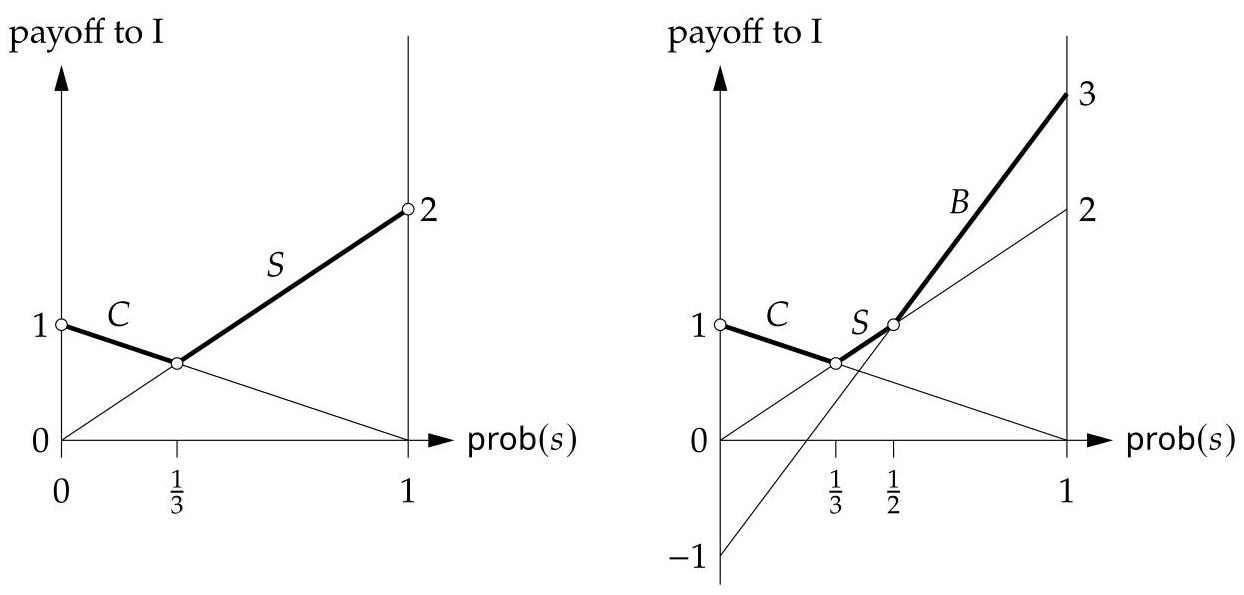
\includegraphics[width=0.9\textwidth]{images/ch06-fig17.jpg}
  \caption{针对图 6.7 中的两个博弈，参与者 II 的混合策略下参与者 I 的期望效用的上包络。白色圆圈表示作为均衡一部分的参与者 II 的混合策略。}
  \label{fig:6.10}
\end{figure}


图\ref{fig:6.10}展示了图\ref{fig:6.7}中两个博弈的上包络图。该图绘制了一个参与者的期望效用与另一个参与者的混合策略之间的关系。当混合策略由单一概率决定时，我们通常会使用这种方法，这适用于参与者只有两种纯策略的情况。在这个例子中，在两个博弈中参与者II都只有两种策略 \(c\) 和 \(s\) ，她的混合策略是$(1 - q, q)$。横轴表示参与者II采用第二种纯策略 \(s\) 的概率 \(q = \operatorname{prob}\left( s\right)\) 。在纵轴方向上，我们绘制了另一个参与者(这里是参与者I)对于他的每种纯策略所得到的期望效用。

首先考虑左边的博弈，其中参与者I只有两种策略 \(C\) 和 \(S\) 。对于 \(C\) ，他针对$(1 - q, q)$的期望效用是 \(1 - q\) ，对于 \(S\) ，期望效用是 \({2q}\) 。上包络是得到的两条线中的最大值，用粗线表示。

右边的博弈中参与者 \(\mathrm{I}\) 有一个额外的策略 \(B\) ，在左列 \(c\) (其中 \(q = 0\) )下的效用为 -1，在右列 \(s\) (其中 \(q = 1\) )下的效用为3。对于 \(q \in  \left\lbrack  {0,1}\right\rbrack\) ，得到的期望效用是 \(- \left( {1 - q}\right)  + {3q}\) ，即 \({4q} - 1\) 。当 \(q \geq  \frac{1}{2}\) 时，这个期望效用成为上包络的新部分，因为当 \(q = \frac{1}{2}\) 时，行 \(S\) 和 \(B\) 的期望效用等于1，此时两条线相交，并且当 \(q > \frac{1}{2}\) 时，行 \(B\) 的期望效用严格优于其他行。

根据以下用于构建上包络的球门柱法，描述期望效用的线特别容易通过图形方式获得:

\begin{itemize}
\item 确定一个只有两种纯策略的参与者(这里是参与者II)。
\end{itemize}

\begin{itemize}
\item 沿水平轴从0到1绘制参与者第二个策略的概率，这里 \(q = \operatorname{prob}\left( s\right)\) 。这就定义了参与者II的混合策略$(1 - q, q)$。这样，区间 \(\left\lbrack  {0,1}\right\rbrack\) 中对应 \(q\) 的左端点0对应参与者II在收益表中的左策略，右端点1对应其右策略。
\end{itemize}

\begin{itemize}
\item 在区间 \(\left\lbrack  {0,1}\right\rbrack\) 的每个端点处竖立一条垂直线(“球门柱”)。
\end{itemize}

\begin{itemize}
\item 对于另一个参与者(即参与者I)的每个纯策略，执行以下操作:在左球门柱上，将参与者I对抗参与者II左策略的收益标记为球门柱上的一个高度，同样在右球门柱上标记参与者I对抗参与者II右策略的收益；然后用一条直线连接这两个高度。对于行 \(C\) ，左右高度分别为1和0；对于行 \(S\) ，分别为0和2；对于行 \(B\) (仅适用于右侧博弈)，分别为 -1和3。这些恰好是收益矩阵中参与者I所在行的元素。
\end{itemize}

%\section{所绘制直线的最大值就是上包络}

这种构造方法可行，特别是能得到期望效用的直线，这是由于上述图5.4中对线段的代数描述。即，考虑某一行，参与者 \(\mathrm{I}\) 的收益为 \(a\) 和 \(b\) ，例如行 \(B\) 的 \(a =  - 1\) 和 \(b = 3\) 。那么他对抗混合策略$(1 - q, q)$的期望效用为 \(\left( {1 - q}\right) a + {qb}\) 。这个期望效用是球门柱图中的垂直坐标(“高度”)，而水平坐标就是 \(q\) 。球门柱上的两个端点坐标为$(0, a)$和$(1, b)$，连接它们所绘制的线段由 \(\left( {1 - q}\right) \left( {0,a}\right)  + q\left( {1,b}\right)\) (其中 \(q \in  \left\lbrack  {0,1}\right\rbrack\) )组成，也就是所声称的 \(\left( {q,\left( {1 - q}\right) a + {qb}}\right)\) 这些点。

在图\ref{fig:6.1}0的左图中，行 \(C\) 和 \(S\) 的两条期望效用线显然恰好相交于参与者 \(\mathrm{I}\) 对这两行无差异的地方，即 \(q = \frac{1}{3}\) 时。然而，该图不仅给出了关于这种无差异的信息，还给出了参与者I的一般偏好信息:参与者I的任何最优反应纯策略显然是描述期望效用的所有直线中最上方的线段。这里，当 \(0 \leq  q \leq  \frac{1}{3}\) 时，行 \(C\) 是最优反应；当 \(\frac{1}{3} \leq  q \leq  1\) 时，行 \(S\) 是最优反应，而当 \(q = \frac{1}{3}\) 时，参与者I对 \(C\) 和 \(S\) 无差异。期望效用的上包络是描述不同纯策略期望效用的直线的最大值，在图中用粗线段表示。因此，用粗线标记这个上包络是球门柱法的最后一步。

当一个参与者有两个以上的纯策略时，上包络特别有用，因为退化博弈的混合策略纳什均衡无论如何都可以通过“差分技巧”快速确定。考虑图\ref{fig:6.1}0右侧的上包络图，它对应图\ref{fig:6.7}中的退化博弈。参与者 \(\mathrm{I}\) 的额外策略 \(B\) 给出了一条从左端点高度 -1 连接到右端点高度 3 的线段，这表明对于所有的 \(q\) ， \(B\) 都是最优反应，使得 \(\frac{1}{2} \leq  q \leq  1\) ，并且当 \(q = \frac{1}{2}\) 时，参与者在 \(S\) 和 \(B\) 之间无差异。上包络由参与者 I 的三个纯策略 \(C,S\) 和 \(B\) 对应的三条线段组成。此外，参与者 \(\mathrm{I}\) 在任意两个这样的策略之间无差异的点只有两个，即当 \(q = \frac{1}{3}\) 时，在 \(C\) 和 \(S\) 之间；当 \(q = \frac{1}{2}\) 时，在 \(S\) 和 \(B\) 之间。这两个点在上包络上用小圆圈表示，它们给出了参与者 II 的仅有的两个混合策略概率，在这些概率下参与者 I 可以在两个纯策略之间进行混合( \(q = 0\) 对应的小圆圈对应纯均衡策略 \(c\) )。在 \(C\) 和 \(B\) 之间还有第三种无差异情况，即当 \(q = \frac{2}{5}\) 时， \(C\) 和 \(B\) 对应的两条线相交，但这个交点在 \(S\) 对应的线下方，因此不在上包络上。因此，这个交点不需要作为参与者 I 在两行 \(C\) 和 \(B\) 之间进行混合的可能的混合策略均衡来研究，因为它们不是最优反应。

给定参与者 I 的这些混合策略候选，我们可以如前一节所述，使用差分技巧快速找出这两个相应的纯策略是否可以以及如何混合，以使参与者 II 无差异。

因此，上包络限制了需要作为可能的均衡混合策略进行测试的策略对。例如，练习~\ref{exer:6.5} 描述了一个退化博弈。在这里，参与者 I 有两个策略，上包络描述了参与者 II 针对参与者 I 的混合策略 $(1 - p, p)$ 的期望效用。因为参与者 II 有五个纯策略，上包络最多可能由五条线段组成；如果参与者 II 的某些纯策略永远不是最优反应，线段可能会更少。因此，在上包络上线段连接的交点最多有四个，在这些点上参与者 II 在她对应的两个策略之间无差异，并且可以在它们之间进行混合。如果没有上包络，需要检查的可能是参与者 II 在均衡中混合的纯策略对不是四个，而是十个(即从五个中选两个的不同方式)，这将需要进行更繁琐的研究。

\(\Rightarrow\) 练习~\ref{exer:6.2} 也可以用上包络方法解决。对于像练习~\ref{exer:6.5} 中的较大博弈，这种方法特别有帮助。

原则上，上包络图也定义了针对在两个以上纯策略之间进行混合的混合策略的期望效用。在这种情况下，这个图更难绘制和可视化，因为它需要更高的维度。第 9 章的图 9.2 展示了一个例子，我们将进一步开发上包络方法来寻找均衡。

\(\Rightarrow\) 简单的练习~\ref{exer:6.6} 有助于通过上包络图理解(被占优)策略。

\section{退化博弈}   \label{sec6.8}

在本节中，我们将处理那些需要更仔细分析才能找到其所有均衡的博弈。我们将完全分析一个例子，然后给出适用于像这个例子中的退化博弈的定义。然后我们讨论更大的博弈，并给出当一个退化博弈何时适用的一般定义\ref{def:6.7}。

图\ref{fig:6.11}是图4.3中威胁博弈的策略形式，其中包含了最优反应的效用。它与性别战博弈类似，都有两个纯策略均衡，这里是$(T, l)$和$(B, r)$。和性别战博弈一样，我们预计会存在一个额外的混合策略均衡，实际上也确实存在。假设这个均衡由参与者 \(\mathrm{I}\) 的混合策略$(1 - p, p)$和参与者II的混合策略$(1 - q, q)$给出。通过差分技巧得到 \(q = \frac{1}{2}\) ，使得参与者 \(\mathrm{I}\) 在 \(T\) 和 \(B\) 之间无差异，从而可以进行混合；对于参与者I，差分技巧得到 \(p = 0\) ，使得参与者II在 \(l\) 和 \(r\) 之间无差异。

更详细地说，如果参与者 \(I\) 分别以概率 \(1 - p\) 和 \(p\) 选择 \(T\) 和 \(B\) ，那么参与者II选择策略 \(l\) 的期望效用是 \(3\left( {1 - p}\right)\) ，选择 \(r\) 的期望效用是 \(3\left( {1 - p}\right)  + {2p}\) ，所以只有当 \(p = 0\) 时，她在 \(l\) 和 \(r\) 之间才无差异。实际上，由于 \(r\) 弱占优 \(l\) ，并且当参与者I选择 \(B\) 时，参与者II选择 \(r\) 的效用更大，所以 \(B\) 以任何正概率出现都会使 \(r\) 成为参与者II的唯一最优反应(而对于 \(r\) ， \(B\) 是参与者 \(\mathrm{I}\) 的唯一最优反应)。因此， \(B\) 以正概率出现的唯一均衡是纯策略均衡$(B, r)$。

\begin{figure}[htbp]
  \centering
  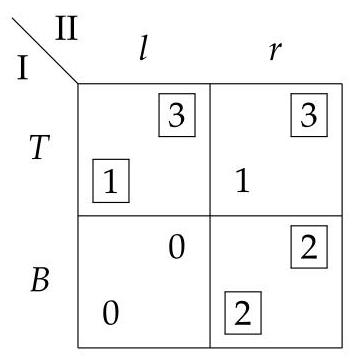
\includegraphics[width=0.3\textwidth]{images/ch06-fig18.jpg}
  \caption{威胁博弈的策略形式，这是一个退化博弈。}
  \label{fig:6.11}
\end{figure}


因此，该博弈的一个混合策略均衡是 \(\left( {\left( {1,0}\right) ,\left( {\frac{1}{2},\frac{1}{2}}\right) }\right)\) 。然而，在这个均衡中，只有参与者II使用了恰当的混合策略，而参与者I选择了纯策略 \(T\) 。最优反应条件要求参与者II在她的纯策略 \(l\) 和 \(r\) 之间无差异，因为这两个策略都以正概率出现，这意味着正如前面所述， \(T\) 以概率1出现。然而，对于参与者I来说，最优反应条件要求 \(T\) 的期望效用最大，这不一定与 \(B\) 的期望效用相同，因为 \(B\) 出现的概率为零！也就是说，我们用来确定参与者II的混合策略$(1 - q, q)$为 \(q = \frac{1}{2}\) 的参与者 \({\mathrm{I}}^{\prime }\mathrm{s}\) 在 \(T\) 和 \(B\) 之间无差异这一条件太强了。我们只需要 \(T\) 是对这个混合策略的最优反应，所以参与者I选择 \(T\) 时期望效用为1，至少要和他选择 \(B\) 时期望效用 \({2q}\) 一样大，即 \(1 \geq  {2q}\) 。换句话说，等式 \(1 = {2q}\) 必须用一个不等式来代替。

不等式 \(1 \geq  {2q}\) 等价于 \(0 \leq  q \leq  \frac{1}{2}\) 。对于 \(q\) 的这些可能取值，我们得到了一个无限的均衡集合 \(\left( {\left( {1,0}\right) ,\left( {1 - q,q}\right) }\right)\) 。 \(q\) 的两个极端情况，即 \(q = 0\) 和 \(q = \frac{1}{2}\) ，分别给出了纯策略均衡$(T, l)$和我们之前找到的混合策略纳什均衡 \(\left( {\left( {1,0}\right) ,\left( {\frac{1}{2},\frac{1}{2}}\right) }\right)\) 。

注意:至少有一个参与者使用非纯策略的混合策略的均衡总是被称为混合策略纳什均衡。此外，当我们想要找到一个博弈的“所有混合策略纳什均衡”时，我们通常会把纯策略均衡也包括在内(无论如何，纯策略均衡很容易找到)。

所描述的均衡集(其中参与者 II 从某个区间中选择混合策略概率 \(q\) )可以从这个博弈中参与者 II 选择 \(l\) 所构成的可能“威胁”来直观理解(在图 4.3(a) 的博弈树中，参与者 I 选择 \(B\) 后会出现不理想的结果)。首先， \(r\) 弱占优 \(l\) ，因此如果参与者 I 有任何正概率忽视该威胁并选择 \(B\) ，那么参与者 II 选择 \(l\) 的威胁就无法作为最优反应持续下去，所以任何参与者 II 选择 \(l\) 的均衡都要求参与者 I 选择 \(B\) 的概率 \(p\) 为零。其次，如果参与者 I 选择 \(T\) ，那么参与者 II 在 \(l\) 和 \(r\) 之间无差异，原则上她可以选择任何策略，但为了维持威胁， \(T\) 必须是最优反应，这要求选择 \(l\) 的概率 \(1 - q\) 足够高。当 \(1 - q = \frac{1}{2}\) 时，参与者 I 在 \(T\) 和 \(B\) 之间无差异(因此 \(T\) 仍然是最优的)。只要 \(1 - q \geq  \frac{1}{2}\) ，威胁就会起作用。换句话说，只要产生不理想结果的受威胁行动的概率足够高，即使该行动不确定，“威胁”也能奏效。

根据以下定义，图\ref{fig:6.11} 中的博弈是“退化的”，这就导致了该博弈的复杂性。

\begin{definition}  \label{def:6.6}  %定义 6.
  如果某个参与者的一个纯策略对应另一个参与者的两个纯最优反应，则称该 \(2 \times  2\) 博弈为退化博弈。  
\end{definition}


退化博弈分析起来很复杂，因为一个参与者可以使用纯策略(如威胁博弈中的 \(T\))，使得另一个参与者可以在她的两个最优反应之间进行混合，但混合策略的概率不必满足另一个参与者在其策略之间无差异的等式。取而代之的是，只需满足第一个参与者的纯策略是最优反应的不等式即可。请注意，上述等式以及不等式都是最优反应条件(命题\ref{prop:6.1})的结果。

\(\Rightarrow\) 练习~\ref{exer:6.7} 是关于一个退化博弈的。

\begin{figure}[htbp]
  \centering
  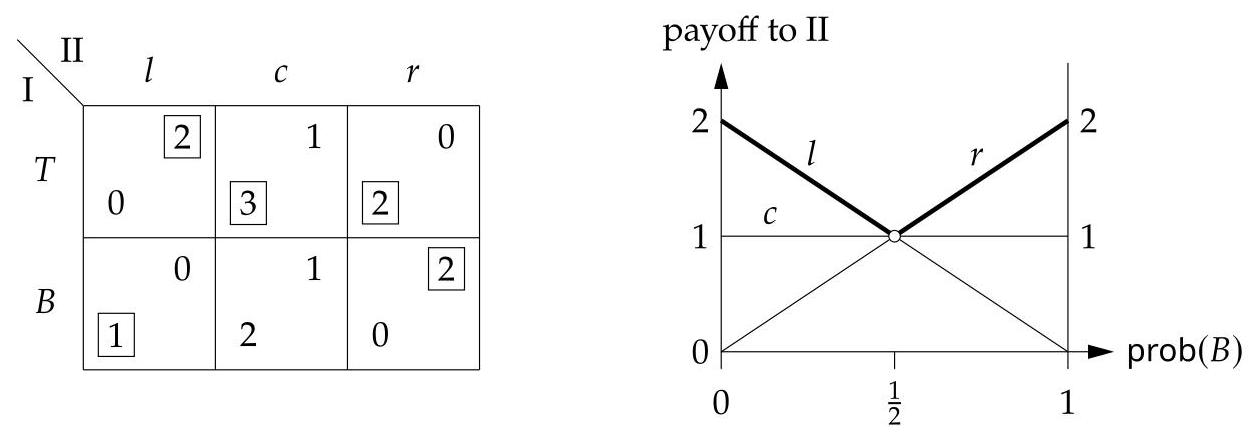
\includegraphics[width=0.9\textwidth]{images/ch06-fig19.jpg}
  \caption{退化 $2 \times 3$ 博弈以及参与者 II 的期望效用上包络。}
  \label{fig:6.12}
\end{figure}


退化现象在更大规模的博弈中也会出现，这需要更一般的定义。考虑图 6.12 中的 \(2 \times  3\) 博弈。每个纯策略都有唯一的最优反应，因此定义 6.6 中的条件不成立。这个博弈没有纯策略均衡，所以两个参与者都必须使用混合策略。我们应用上包络法，将参与者 II 的收益绘制为参与者 I 选择 \(B\) 的概率的函数，如图 6.12 右侧所示。在这里，期望效用线在一个点相交，当参与者 I 使用混合策略 \(\left( {\frac{1}{2},\frac{1}{2}}\right)\) 时，参与者 II 的所有三个纯策略都是最优反应。

我们应该如何分析这个博弈呢？显然，只有当两个参与者都采用混合策略时才会达到均衡，这要求参与者 \(\mathrm{I}\) 使用混合策略 \(\left( {\frac{1}{2},\frac{1}{2}}\right)\) 。然后必须使参与者 I 无差异，为了实现这一点，参与者 II 可以在她的三个最优反应 \(l,c\) 和 \(r\) 之间进行混合。现在我们遇到了与之前威胁博弈中相同的问题，即自由度太大:参与者 II 的三个概率，设为 \({y}_{l},{y}_{c}\) 和 \({y}_{r}\)，必须选择使得 \({y}_{l} + {y}_{c} + {y}_{r} = 1\)，并且使得参与者 \(\mathrm{I}\) 在他的纯策略 \(T\) 和 \(B\) 之间无差异，这给出了等式 \(3{y}_{c} + 2{y}_{r} = {y}_{l} + 2{y}_{c}\)。这是三个未知数受两个方程约束，解是不确定的。

我们给出一种找出所有可能概率的方法，该方法可以推广到像这里这样三个概率仅受两个线性方程约束的情形。首先，对描述另一个参与者期望效用无差异的方程 \(3{y}_{c} + 2{y}_{r} = {y}_{l} + 2{y}_{c}\) 中概率的系数进行整理，使得每个概率仅出现一次且其系数为正，在此得到方程 \({y}_{c} + 2{y}_{r} = {y}_{l}\) 。在这三个概率中，通常有两个出现在方程的一侧，另一个出现在另一侧。通过将方程中包含两个概率那一侧的任意一个概率设为零，即可得到该方程的“极端解”，在此即 \({y}_{c} = 0\) 或 \({y}_{r} = 0\) 。在前一种情况下，对于 \(\left( {{y}_{l},{y}_{c},{y}_{r}}\right)\) 可得到解 \(\left( {\frac{2}{3},0,\frac{1}{3}}\right)\) ；在后一种情况下，可得到解 \(\left( {\frac{1}{2},\frac{1}{2},0}\right)\) 。这意味着在任何均衡中 \(0 \leq  {y}_{c} \leq  \frac{1}{2}\) (同理 \(\left. {0 \leq  {y}_{r} \leq  \frac{1}{3}}\right)\) )。通过选择 \({y}_{c} \in  \left\lbrack  {0,\frac{1}{2}}\right\rbrack\) 作为自由参数，其余概率由 \({y}_{l} = {y}_{c} + 2{y}_{r} = {y}_{c} + 2\left( {1 - {y}_{l} - {y}_{c}}\right)  = 2 - 2{y}_{l} - {y}_{c}\) 或 \({y}_{l} = \frac{2}{3} - \frac{1}{3}{y}_{c}\) 以及 \({y}_{r} = 1 - {y}_{l} - {y}_{c} = 1 - \left( {\frac{2}{3} - \frac{1}{3}{y}_{c}}\right)  - {y}_{c} = \frac{1}{3} - \frac{2}{3}{y}_{c}\) 给出。

找出参与者 II 未完全确定的混合策略概率的极端解的另一种方法是，简单地忽略三个最优反应中的一个，然后应用差分技巧:假设参与者 II 仅使用其最优反应 \(l\) 和 \(c\) 。那么，为了使参与者 I 达到无差异，差分技巧给出 \(l,c,r\) 的概率为 \(\left( {\frac{1}{2},\frac{1}{2},0}\right)\) 。如果参与者 II 仅使用其最优反应 \(l\) 和 \(r\) ，差分技巧给出混合策略 \(\left( {\frac{2}{3},0,\frac{1}{3}}\right)\) 。这正是刚刚描述的两种混合策略。如果参与者 II 仅使用其最优反应 \(c\) 和 \(r\) ，那么差分技巧就不起作用了，因为参与者 I 对 \(c\) 和 \(r\) 的最优反应始终是 \(T\) 。

以下是一般 \(m \times  n\) 博弈的退化定义。

\begin{definition}[退化博弈] \label{def:6.7} %定义 6.7
    如果某个参与者有一个混合策略，该策略恰好对 \(k\) 个纯策略赋予正概率，使得另一个参与者对该混合策略有超过 \(k\) 个纯最优反应，那么这个两人博弈就被称为退化博弈。
\end{definition}


在退化博弈中，具有“过多”最优反应的混合策略会产生我们在上述例子中所描述的困难。相比之下，考虑博弈是非退化的“正常”情形。

\bigskip
\noindent

\begin{proposition}\label{prop:6.8} %命题 6.8
    在任何非退化的两人博弈的均衡中，两个参与者使用的混合策略所混合的纯策略数量相同。
\end{proposition}


\(\Rightarrow\) 你需要在练习~\ref{exer:6.8} 中给出命题~\ref{prop:6.8} 的简单且有启发性的证明。

换句话说，在非退化博弈中，我们有纯策略均衡(两个参与者都恰好使用一种纯策略)，或者混合策略均衡(两个参与者都恰好混合使用两种策略)，或者均衡中两个参与者都恰好混合使用三种策略，依此类推。一般来说，在非退化博弈中，两个参与者都恰好混合使用 \(k\) 种纯策略。这些策略中的每一种都有一个概率，并且这些概率要满足 \(k\) 个方程，以使另一个参与者在其纯策略之间无差异:其中一个方程表示概率之和为 1，另外 \(k - 1\) 个方程表示另一个参与者的第一种和第二种、第二种和第三种，依此类推，直到第 $(k - 1)$ 种和第 \(k\) 种策略之间的期望效用相等。这些方程有唯一解。(可以证明，非唯一解只可能出现在退化博弈中。)需要检查这些解是否具有均衡性质:得到的概率必须是非负的，并且另一个参与者未使用的纯策略的期望效用不能更高。正如我们所证明的，在退化博弈中，通过使另一个参与者的期望效用相等来找到混合策略的概率不再能得到唯一解。

我们是否应该关注退化博弈呢？从某种意义上说，当考虑{\color{red}策略型}博弈，并且收益表的每个单元格都源于该博弈所建模的交互情境的不同情况时，可以忽略退化博弈。在这种情况下，两个收益相同的可能性“很小”，而这是对一种纯策略有两种纯最优反应的必要条件，而这也是退化博弈可能出现的唯一情况。收益的微小变化会导致另一个参与者有唯一的偏好。同样，定义期望效用上包络的两条以上的线在一点相交的可能性很小，或者针对混合三种纯策略的混合策略(如在图 9.2 中的两个平面)的三个以上的期望效用平面在一点相交的可能性也很小，依此类推。换句话说，策略形式下的“一般”(或“几乎所有”)博弈是非退化的。另一方面，{\color{red}对于博弈树型的博弈而言}，退化的可能性非常大，因为博弈树的一个收益会在策略形式中反复出现，如威胁博弈所示。

我们以一个有用的命题作为结论，该命题可用于寻找退化博弈的所有均衡。在图\ref{fig:6.11}的威胁博弈中，有两个均衡 \(\left( {\left( {1,0}\right) ,\left( {1,0}\right) }\right)\) 和 \(\left( {\left( {1,0}\right) ,\left( {\frac{1}{2},\frac{1}{2}}\right) }\right)\) ，本质上是通过“忽略”退化得到的。这两个均衡中参与者 I 的策略相同，均为 (1,0)。类似地，图\ref{fig:6.12}中的博弈有两个混合策略纳什均衡 \(\left( {\left( {\frac{1}{2},\frac{1}{2}}\right) ,\left( {\frac{1}{2},\frac{1}{2},0}\right) }\right)\) 和 \(\left( {\left( {\frac{1}{2},\frac{1}{2}}\right) ,\left( {\frac{2}{3},0,\frac{1}{3}}\right) }\right)\) ，它们同样具有参与者 \(\mathrm{I}\) 的相同策略。

以下命题指出，在两人博弈中，具有一个参与者相同策略的两个混合策略纳什均衡可以通过凸组合相结合，以得到更多的均衡，就像上述例子中的情况一样。在该命题中，参与者 II 的策略 \(y\) 是固定的，但当参与者 I 的策略固定时，情况类似。在这里固定策略很重要，因为均衡集一般不是凸集。


\begin{proposition}\label{prop:6.9} %命题6.9
    考虑一个双矩阵博弈$(A, B)$，其混合策略集为 \(X\) 和 \(Y\) ，如(6.6)所示。设$(x, y)$和 \(\left( {\widehat{x},y}\right)\) 是该博弈的均衡，其中 \(x,\widehat{x} \in  X\) 且 \(y \in  Y\) 。那么对于任意 \(p \in  \left\lbrack  {0,1}\right\rbrack\)， \(\left( {x\left( {1 - p}\right)  + \widehat{x}p}\right) ,y)\) 也是该博弈的一个均衡。
\end{proposition}

\begin{proof}
设 \(\bar{x} = x\left( {1 - p}\right)  + \widehat{x}p\) 。显然， \(\bar{x} \in  X\) ，因为对于参与者I的所有纯策略 \(i\) ，都有 \({\bar{x}}_{i} \geq  0\) ，并且
\begin{equation}
\label{eq:6.23}
\mathbf{1}^{\top} \bar{x} 
= \mathbf{1}^{\top} \big( x (1-p) + \widehat{x} p \big) 
= \mathbf{1}^{\top} x (1-p) + \mathbf{1}^{\top} \widehat{x} p 
= (1-p) + p = 1.
\end{equation}


如果 \(\bar{x}\) 是对 \(y\) 的最优反应，反之亦然，那么 \(\left( {\bar{x},y}\right)\) 这一对就是一个均衡。对于参与者 \(\mathrm{I}\) 的任何混合策略 \(\widetilde{x}\) ，我们有 \({x}^{\top }{Ay} \geq  {\widetilde{x}}^{\top }{Ay}\) 和 \({\widehat{x}}^{\top }{Ay} \geq  {\widetilde{x}}^{\top }{Ay}\) ，因此

\[
{\bar{x}}^{\top }{Ay} = \left( {1 - p}\right) {x}^{\top }{Ay} + p{\widehat{x}}^{\top }{Ay} \geq  \left( {1 - p}\right) {\widetilde{x}}^{\top }{Ay} + p{\widetilde{x}}^{\top }{Ay} = {\widetilde{x}}^{\top }{Ay},
\]

这表明 \(\bar{x}\) 是对 \(y\) 的最优反应。换句话说，这些不等式成立是因为它们在凸组合下保持不变。类似地， \(y\) 是对 \(x\) 和 \(\widehat{x}\) 的最优反应，即对于任何 \(\widetilde{y} \in  Y\) ，我们有 \({x}^{\top }{By} \geq  {x}^{\top }B\widetilde{y}\) 和 \({\widehat{x}}^{\top }{By} \geq  {\widehat{x}}^{\top }B\widetilde{y}\) 。再次，取凸组合表明 \({\bar{x}}^{\top }{By} \geq  {\bar{x}}^{\top }B\widetilde{y}\) 。因此，如所声称的， \(\left( {\bar{x},y}\right)\) 是一个均衡。
\end{proof}

我们回到图\ref{fig:6.12}的例子来说明命题6.9:这个博弈有两个均衡$(x, y)$和 \(\left( {x,\widehat{y}}\right)\) ，其中 \(x = \left( {\frac{1}{2},\frac{1}{2}}\right) ,y = \left( {\frac{1}{2},\frac{1}{2},0}\right)\) 且 \(\widehat{y} = \left( {\frac{2}{3},0,\frac{1}{3}}\right)\) ，所以这就是命题6.9的情况，只是这两个均衡中参与者I的混合策略相同，而不是参与者II的。因此，对于 \(y\) 和 \(\widehat{y}\) 的任何凸组合 \(\bar{y}\) ， \(\left( {x,\bar{y}}\right)\) 都是一个均衡。均衡$(x, y)$和 \(\left( {x,\widehat{y}}\right)\) 是“极端的”，因为 \(y\) 和 \(\widehat{y}\) 的概率尽可能多地为零，这意味着 \(y\) 和 \(\widehat{y}\) 是均衡策略线段 \(\bar{y} = y\left( {1 - p}\right)  + \widehat{y}p\) 的端点(即 \(\left( {x,\bar{y}}\right)\) 是一个均衡)。

\(\Rightarrow\) 借助命题\ref{prop:6.9}，求出图\ref{fig:6.11}中威胁博弈的均衡集。

\section{延伸阅读}   \label{sec6.9}

在第\ref{sec6.2}节中，监管博弈被用于引入混合策略。监管博弈是博弈论的一个应用领域；例如，可参见Avenhaus和Canty (1996)。

纳什(1951)的开创性论文定义了有限博弈中的“均衡点”并证明了它们的存在性。如前所述，纳什(1951，第287页)称最优反应条件为“显而易见的”，但它对于寻找混合策略纳什均衡至关重要。纳什的“均衡点”现在被普遍称为“纳什均衡”，这是本书通篇所考虑的均衡概念，第12章中相关均衡的推广情况除外。关于混合策略均衡的教科书式处理，可参阅奥斯本(2004，第4章)或马斯勒、索兰和扎米尔(2013，第5章)。

上包络的使用似乎是业内常识，而且无论如何都很直接。关于定义6.7，可参阅范·达默(1987，第52页)；关于两人博弈退化条件的详细比较(所有这些条件都与此定义等价)，可参阅冯·施滕格尔(2021)。

\section{第6章练习}  \label{sec6.10}

\bigskip
\noindent
\begin{exercise}\label{exer:6.1}
设 \(x \in  {\mathbb{R}}^{m}\) 和 \(y \in  {\mathbb{R}}^{n}\) ，并记住所有向量都是列向量。如果 \(m = n\) ， \({x}^{\top }y\) 和 \(x{y}^{\top }\) 之间的差异是什么？如果 \(m \neq  n\) 呢？
\end{exercise}

\bigskip
\noindent
\begin{exercise}\label{exer:6.2}
找出这个 \(3 \times  2\) 博弈的所有混合策略纳什均衡(这总是包括任何纯策略均衡)。

\begin{center}
\begin{tabular}{|c|c|c|}
\hline
\diagbox{I}{II} & $l$ & $r$ \\
\hline
$T$ & $0\;\;1$ & $6\;\;0$ \\
\hline
$M$ & $2\;\;0$ & $5\;\;2$ \\
\hline
$B$ & $3\;\;3$ & $3\;\;4$ \\
\hline
\end{tabular}
\end{center}


\end{exercise}

\bigskip
\noindent
\begin{exercise}\label{exer:6.3}
考虑练习~\ref{exer:4.5} 中的三人博弈树。回想一下，混合策略纳什均衡中的部分或所有策略可能是纯策略。

(a) 以下陈述是对还是错？直接用博弈树来论证是最容易的。

对于参与者I、II或III中的每一个，该博弈都有一个混合策略纳什均衡，其中该参与者采用的混合策略不是纯策略。

(b) 以下陈述是对还是错？请解释。

在该博弈的每个混合策略纳什均衡中，参与者I、II或III中至少有一个采用纯策略。
\end{exercise}

\bigskip
\noindent
\begin{exercise}\label{exer:6.4}
在这个 \(2 \times  2\) 博弈中， \(A,B,C,D\) 是参与者I的收益，它们是实数，且任意两个都不相等。类似地， \(a,b,c,d\) 是参与者II的收益，它们也是实数，且任意两个也不相等。
\begin{center}
\begin{tabular}{|c|c|c|}
\hline
\diagbox{I}{II} & $left$ & $right$ \\
\hline
$Top$ & $A\;\;a$ & $B\;\;b$ \\
\hline
$Bottom$ & $C\;\;c$ & $D\;\;d$ \\
\hline
\end{tabular}
\end{center}

(a) 在什么条件下，这个博弈有一个不是纯策略均衡的混合策略纳什均衡？

[提示:考虑最优反应的可能模式以及由此产生的可能的占优关系，并通过比较收益来表达，例如 \(A > C\) 。]

(b) 在(a)中的什么条件下，这是该博弈的唯一均衡？

(c) 考虑(b)中的一种情况，分别计算在均衡状态下选择“上”和“下”的概率 \(1 - p\) 和 \(p\) ，以及选择“左”和“右”的概率 \(1 - q\) 和 \(q\) 。

(d) 对于(c)中的解，用收益参数给出商 \(\left( {1 - p}\right) /p\) 和 \(\left( {1 - q}\right) /q\) 的简单公式。尽量使该公式的分母和分子均为正数。

(e) 证明:若参与者I的收益 \(A\) 和 \(C\) 分别被替换为 \(A + E\) 和 \(C + E\) (其中 \(E\) 为某个常数)，且若参与者II的收益 \(a\) 和 \(b\) 分别被替换为 \(a + e\) 和 \(b + e\) (其中 \(e\) 为某个常数)，则混合策略纳什均衡(mixed equilibrium)策略不会改变。
\end{exercise}

\bigskip
\noindent
\begin{exercise}\label{exer:6.5}
考虑以下 \(2 \times  5\) 博弈:

\begin{center}
\begin{tabular}{|c|c|c|c|c|c|}
\hline
\diagbox{I}{II} & $a$ & $b$ & $c$ & $d$ & $e$ \\
\hline
$T$ & $0\;\;2$ & $2\;\;4$ & $1\;\;3$ & $0\;\;5$ & $3\;\;0$ \\
\hline
$B$ & $1\;\;7$ & $0\;\;4$ & $4\;\;5$ & $1\;\;0$ & $0\;\;8$ \\
\hline
\end{tabular}
\end{center}



(a) 绘制参与者 II 所有策略 \(a,b,c,d,e\) 的期望效用，以参与者 I 选择策略 \(B\) 的概率 \(p\) 来表示。根据该概率 \(p\) 指出参与者 II 的最优反应。

(b) 利用 (a) 中的图表，找出该博弈的所有混合(包括纯策略)均衡。
\end{exercise}

\bigskip
\noindent
\begin{exercise}\label{exer:6.6}
考虑图 3.2(b) 中的产品质量博弈。

(a) 两次使用“门柱”方法，绘制参与者 I 针对参与者 II 混合策略的最优反应收益的上包络，反之亦然。

(b) 解释这些图表中哪一个表明一个纯策略占优于另一个纯策略。

(c) 解释该图表如何表明，如果一个纯策略 \(s\) 占优于策略 \(t\) ，那么 \(t\) 永远不是最优反应。
\end{exercise}

\begin{exercise}\label{exer:6.7}
找出下面这个退化博弈的所有均衡。该博弈是图 6.2 所示监管博弈的一个变体。不同之处在于，参与者 II（即被监管者）即使在未被监管的情况下(参与者 \(\mathrm{I}\) 选择 \(T\) )，若采取非法行为(选择 \(r\) )也不会获得任何收益。
\begin{center}
\begin{tabular}{|c|c|c|}
\hline
\diagbox{I}{II} & $l$ & $r$ \\
\hline
$T$ & $0\;\;0$ & $-10\;\;0$ \\
\hline
$B$ & $-1\;\;0$ & $-6\;\;-90$ \\
\hline
\end{tabular}
\end{center}



\end{exercise}

\begin{exercise}\label{exer:6.8}
证明命题~\ref{prop:6.8}。
\end{exercise}
